%%%%%%%%%%%%%%%%%%%%%%%%%%%%%%%%%%%%%%%%%
% Masters/Doctoral Thesis 
% LaTeX Template
% Version 2.5 (27/8/17)
%
% This template was downloaded from:
% http://www.LaTeXTemplates.com
%
% Version 2.x major modifications by:
% Vel (vel@latextemplates.com)
%
% This template is based on a template by:
% Steve Gunn (http://users.ecs.soton.ac.uk/srg/softwaretools/document/templates/)
% Sunil Patel (http://www.sunilpatel.co.uk/thesis-template/)
%
% Template license:
% CC BY-NC-SA 3.0 (http://creativecommons.org/licenses/by-nc-sa/3.0/)
%
%%%%%%%%%%%%%%%%%%%%%%%%%%%%%%%%%%%%%%%%%

%----------------------------------------------------------------------------------------
%	PACKAGES AND OTHER DOCUMENT CONFIGURATIONS
%----------------------------------------------------------------------------------------

\documentclass[
11pt, % The default document font size, options: 10pt, 11pt, 12pt
%oneside, % Two side (alternating margins) for binding by default, uncomment to switch to one side
english, % ngerman for German
singlespacing, % Single line spacing, alternatives: onehalfspacing or doublespacing
%draft, % Uncomment to enable draft mode (no pictures, no links, overfull hboxes indicated)
%nolistspacing, % If the document is onehalfspacing or doublespacing, uncomment this to set spacing in lists to single
%liststotoc, % Uncomment to add the list of figures/tables/etc to the table of contents
%toctotoc, % Uncomment to add the main table of contents to the table of contents
%parskip, % Uncomment to add space between paragraphs
%nohyperref, % Uncomment to not load the hyperref package
headsepline, % Uncomment to get a line under the header
%chapterinoneline, % Uncomment to place the chapter title next to the number on one line
%consistentlayout, % Uncomment to change the layout of the declaration, abstract and acknowledgements pages to match the default layout
]{MastersDoctoralThesis} % The class file specifying the document structure

\usepackage[utf8]{inputenc} % Required for inputting international characters
\usepackage[T1]{fontenc} % Output font encoding for international characters

\usepackage{mathpazo} % Use the Palatino font by default

\usepackage[backend=bibtex,style=authoryear,natbib=true]{biblatex} % Use the bibtex backend with the authoryear citation style (which resembles APA)

\addbibresource{example.bib} % The filename of the bibliography

\usepackage[autostyle=true]{csquotes} % Required to generate language-dependent quotes in the bibliography
\usepackage{graphicx}
%----------------------------------------------------------------------------------------
%	MARGIN SETTINGS
%----------------------------------------------------------------------------------------

\geometry{
	paper=a4paper, % Change to letterpaper for US letter
	inner=2.5cm, % Inner margin
	outer=3.8cm, % Outer margin
	bindingoffset=.5cm, % Binding offset
	top=1.5cm, % Top margin
	bottom=1.5cm, % Bottom margin
	%showframe, % Uncomment to show how the type block is set on the page
}

%----------------------------------------------------------------------------------------
%	THESIS INFORMATION
%----------------------------------------------------------------------------------------

\thesistitle{Thesis Title} % Your thesis title, this is used in the title and abstract, print it elsewhere with \ttitle
\supervisor{Prof. Dr. Thomas \textsc{Hanne}} % Your supervisor's name, this is used in the title page, print it elsewhere with \supname
\examiner{} % Your examiner's name, this is not currently used anywhere in the template, print it elsewhere with \examname
\degree{Master of Science in Business Information Systems} % Your degree name, this is used in the title page and abstract, print it elsewhere with \degreename
\author{Kevin \textsc{Saner}} % Your name, this is used in the title page and abstract, print it elsewhere with \authorname
\addresses{} % Your address, this is not currently used anywhere in the template, print it elsewhere with \addressname

\subject{Biological Sciences} % Your subject area, this is not currently used anywhere in the template, print it elsewhere with \subjectname
\keywords{} % Keywords for your thesis, this is not currently used anywhere in the template, print it elsewhere with \keywordnames
\university{Fachhochschule Nordwestschweiz} % Your university's name and URL, this is used in the title page and abstract, print it elsewhere with \univname
\department{\href{https://www.fhnw.ch/en/about-fhnw/schools/business}{School of Business}} % Your department's name and URL, this is used in the title page and abstract, print it elsewhere with \deptname
\faculty{\href{}{}} % Your faculty's name and URL, this is used in the title page and abstract, print it elsewhere with \facname

\AtBeginDocument{
\hypersetup{pdftitle=\ttitle} % Set the PDF's title to your title
\hypersetup{pdfauthor=\authorname} % Set the PDF's author to your name
\hypersetup{pdfkeywords=\keywordnames} % Set the PDF's keywords to your keywords
}

\begin{document}

\frontmatter % Use roman page numbering style (i, ii, iii, iv...) for the pre-content pages

\pagestyle{plain} % Default to the plain heading style until the thesis style is called for the body content

%----------------------------------------------------------------------------------------
%	TITLE PAGE
%----------------------------------------------------------------------------------------

\begin{titlepage}
\begin{center}

\vspace*{.06\textheight}
{\scshape\LARGE \univname\par}\vspace{1.5cm} % University name
\textsc{\Large Master Thesis Proposal}\\[0.5cm] % Thesis type

\HRule \\[0.4cm] % Horizontal line
{\huge \bfseries \ttitle\par}\vspace{0.4cm} % Thesis title
\HRule \\[1.5cm] % Horizontal line
 
\begin{minipage}[t]{0.4\textwidth}
\begin{flushleft} \large
\emph{Author:}\\
\href{}{\authorname} % Author name - remove the \href bracket to remove the link
\end{flushleft}
\end{minipage}
\begin{minipage}[t]{0.4\textwidth}
\begin{flushright} \large
\emph{Supervisor:} \\
\href{}{\supname} % Supervisor name - remove the \href bracket to remove the link  
\end{flushright}
\end{minipage}\\[3cm]
 
\vfill

\large \textit{A thesis proposal submitted in fulfillment of the requirements\\ for the degree of \degreename}\\[0.3cm] % University requirement text
\textit{in the}\\[0.4cm]
\deptname\\[2cm] % Research group name and department name
 
\vfill

{\large \today}\\[4cm] % Date
%\includegraphics{Logo} % University/department logo - uncomment to place it
 
\vfill
\end{center}
\end{titlepage}

%----------------------------------------------------------------------------------------
%	DECLARATION PAGE
%----------------------------------------------------------------------------------------

\begin{declaration}
\addchaptertocentry{\authorshipname} % Add the declaration to the table of contents
\noindent I, \authorname, declare that this thesis titled, \enquote{\ttitle} and the work presented in it are my own. I confirm that:

\begin{itemize} 
\item This work was done wholly or mainly while in candidature for a research degree at this University.
\item Where any part of this thesis has previously been submitted for a degree or any other qualification at this University or any other institution, this has been clearly stated.
\item Where I have consulted the published work of others, this is always clearly attributed.
\item Where I have quoted from the work of others, the source is always given. With the exception of such quotations, this thesis is entirely my own work.
\item I have acknowledged all main sources of help.
\item Where the thesis is based on work done by myself jointly with others, I have made clear exactly what was done by others and what I have contributed myself.\\
\end{itemize}
 
\noindent Signed:\\
\rule[0.5em]{25em}{0.5pt} % This prints a line for the signature
 
\noindent Date:\\
\rule[0.5em]{25em}{0.5pt} % This prints a line to write the date
\end{declaration}

\cleardoublepage

%----------------------------------------------------------------------------------------
%	QUOTATION PAGE
%----------------------------------------------------------------------------------------

\vspace*{0.2\textheight}

\noindent\enquote{\itshape Your brain does not manufacture thoughts. Your thoughts shape neural networks.}\bigbreak

\hfill Deepak Chopra

%----------------------------------------------------------------------------------------
%	ABSTRACT PAGE
%----------------------------------------------------------------------------------------

\begin{abstract}
\addchaptertocentry{\abstractname} % Add the abstract to the table of contents
The Thesis Abstract is written here (and usually kept to just this page). The page is kept centered vertically so can expand into the blank space above the title too\ldots
\end{abstract}

%----------------------------------------------------------------------------------------
%	ACKNOWLEDGEMENTS
%----------------------------------------------------------------------------------------

\begin{acknowledgements}
\addchaptertocentry{\acknowledgementname} % Add the acknowledgements to the table of contents
The acknowledgments and the people to thank go here.
%, don't forget to include your project advisor\ldots
\end{acknowledgements}

%----------------------------------------------------------------------------------------
%	LIST OF CONTENTS/FIGURES/TABLES PAGES
%----------------------------------------------------------------------------------------

\tableofcontents % Prints the main table of contents

\listoffigures % Prints the list of figures

\listoftables % Prints the list of tables

%----------------------------------------------------------------------------------------
%	ABBREVIATIONS
%----------------------------------------------------------------------------------------

\begin{abbreviations}{ll} % Include a list of abbreviations (a table of two columns)

\textbf{DNN} & \textbf{D}eep \textbf{N}eural \textbf{N}etwork\\
\textbf{CNN} & \textbf{C}onvolutional \textbf{N}eural \textbf{N}etwork\\
\textbf{RNN} & \textbf{R}ecurrent \textbf{N}eural \textbf{N}etwork\\
\textbf{GRU} & \textbf{G}ated \textbf{R}ecurrent \textbf{U}nit Network\\
\textbf{LSTM} & \textbf{L}ong \textbf{S}hort \textbf{T}erm \textbf{M}emory\\


\end{abbreviations}

%----------------------------------------------------------------------------------------
%	PHYSICAL CONSTANTS/OTHER DEFINITIONS
%----------------------------------------------------------------------------------------

%\begin{constants}{lr@{${}={}$}l} % The list of physical constants is a three column table

% The \SI{}{} command is provided by the siunitx package, see its documentation for instructions on how to use it

%Speed of Light & $c_{0}$ & \SI{2.99792458e8}{\meter\per\second} (exact)\\
%Constant Name & $Symbol$ & $Constant Value$ with units\\

%\end{constants}

%----------------------------------------------------------------------------------------
%	SYMBOLS
%----------------------------------------------------------------------------------------

%\begin{symbols}{lll} % Include a list of Symbols (a three column table)

%$a$ & distance & \si{\meter} \\
%$P$ & power & \si{\watt} (\si{\joule\per\second}) \\
%Symbol & Name & Unit \\

%\addlinespace % Gap to separate the Roman symbols from the Greek

%$\omega$ & angular frequency & \si{\radian} \\

%\end{symbols}

%----------------------------------------------------------------------------------------
%	DEDICATION
%----------------------------------------------------------------------------------------

\dedicatory{For/Dedicated to/To my\ldots} 

%----------------------------------------------------------------------------------------
%	THESIS CONTENT - CHAPTERS
%----------------------------------------------------------------------------------------

\mainmatter % Begin numeric (1,2,3...) page numbering

\pagestyle{thesis} % Return the page headers back to the "thesis" style

% Include the chapters of the thesis as separate files from the Chapters folder
% Uncomment the lines as you write the chapters

% Chapter 1

\chapter{Introduction} % Main chapter title

\label{1.} % For referencing the chapter elsewhere, use \ref{Chapter1} 

%----------------------------------------------------------------------------------------

% Define some commands to keep the formatting separated from the content 
\newcommand{\keyword}[1]{\textbf{#1}}
\newcommand{\tabhead}[1]{\textbf{#1}}
\newcommand{\code}[1]{\texttt{#1}}
\newcommand{\file}[1]{\texttt{\bfseries#1}}
\newcommand{\option}[1]{\texttt{\itshape#1}}


%----------------------------------------------------------------------------------------


With the rise of the Internet of Things (IoT) and ever more sensors, gadgets and smart devices like smartwatches for fall detection or blood pressure monitoring, or fridges for temperature protective control in use, the amount of available data steadily increases \parencite{Alansari2018}. Simultaneously, the possibilities to use the data to draw conclusions increases. This data is generally used to draw conclusions such as failure of a system or a medical issue, such as a heart attack. These events typically occur very rarely \parencite{Hauskrecht2007}. However, when the number of instances of each class is approximately equal, most machine learning algorithms function best. Problems occur when the number of instances of one class greatly exceeds the number of instances of the other. This issue is very popular in practice, and it can be observed in a variety of fields such as fraud detection, medical diagnosis, oil spillage detection, facial recognition, and so on \parencite{Thabtah2020}. The task of identifying the rare item, event or observation is often referred to as anomaly detection. Typically, the anomalous item translates to problems such as bank fraud or medical problems. Often, the anomaly does not adhere to the common statistical definition of an outlier. Therefore, many outlier detection methods (in particular unsupervised methods) fail on such data \parencite{Hodge2004}

A special disciplin in anomaly detection is to find the anomaly in a time series. The anomaly detection problem for time series is usually formulated as finding outlier data points relative to some standard or usual signal. Time series anomaly detection plays a critical role in automated monitoring systems. It is an increasingly important topic today, because of its wider application in the context of the Internet of Things (IoT), especially in industrial environments. The most popular techniques to find the anomalies are:

\begin{itemize}
	\item Statistical Methods
	\item Support Vector Machines
	\item Clustering 
	\item Density-based Techniques
	\item Neural Networks 
\end{itemize}

Currently Neural Networks are regarded the cutting-edge research. Although first approaches to use artificial neural networks exist since 1969. They are popular in research for only about 15 to 20 years. Neural networks are well-suited for assisting people in solving complex problems in real-world situations. They can learn and model nonlinear and complex relationships between inputs and outputs; make generalizations and inferences; uncover hidden relationships, patterns, and predictions; and model highly volatile data (such as financial time series data) and variances required to predict rare events (such as fraud detection). Since neural networks do not require time intensive feature engineering, but instead learn the features themselves a lot of time can be saved setting up a model compared to traditional machine learning approaches. At the moment, there is a lot of research focussing on neural networks, which is why scientist generally expect further improvements on this kind of technology. This promising outlook is why this research paper also purely focusses on Neural Networks for anomaly detection. Especially Recurrent Neural Networks and Convolutional Neural Networks are investigated and compared.


\section{Definitions}
Following, the most important terms in the context of anomaly detection using neural networks are elaborated and defined. 

\subsection{Univariate, Bivariate and Multivariate Data}
Time series data investigation poses a special disciplin. Generally anomalies in time series are harder to detect for traditional statistical models, since the possibility of long term dependencies exist. Time series data comes in different forms. It is distinguished between univariate, bivariate and multivariate data. Univariate involves the analysis of a single variable while bivariate and multivariate analysis examines two or more variables. One significant difference between time-series and other datasets is that the observations are dependent not only on the components d, but also on the time feature n. Thus, time-series analysis and the statistical methods employed are largely distinct from methods employed for random variables, which assume independence and constant variance of the random variables. Time-series are important to data analysts in a variety of fields such as the economy, healthcare and medical research, trading, engineering, and geophysics. These data are used for forecasting and detecting anomalies.

\subsubsection{Univariate Data}
There is only one variable in this type of data. Because the information only deals with one variable that changes, univariate data analysis is the simplest type of analysis. It is not concerned with causes or relationships, and the primary goal of the analysis is to describe the data and identify patterns.

\subsubsection{Bivariate Data}
This type of data involves two different variables. This type of data analysis is concerned with causes and relationships, and the goal is to determine the relationship between the two variables.

\subsubsection{Multivariate Data}
Multivariate data is defined as data that contains three or more variables. It's similar to bivariate, but there are more dependent variables meaning there is not only one variable that influences the observed beahavior (independent variable) but several. The methods for analyzing this data are determined by the objectives to be met. Regression analysis, path analysis, factor analysis, and multivariate analysis of variance are some of the techniques. Data collected from several sensors installed in a car is an example of a multivariate time-series.

\subsection{Neural Networks}

An Artificial Neural Network (ANN) with several layers between the input and output layers, is known as a Deep Neural Network (DNN). Neural networks come in a variety of shapes and sizes, but they all have the same basic components: neurons, weights and functions. These components work in a similar way as human brains and can be trained just like any other machine learning algorithm.

\subsubsection{Neuron}
Artificial neurons represent the smallest building blocks of neural networks. A neuron usually receives separately weighted inputs which it sums. The sum is then passed through the activation function to calculate the output of the neuron. When training a neural network, the input weights are adjusted by the optimizer function to improve accuracy of the given task e.g. classification.

\subsubsection{Layer}
In neural networks three different kind of layers are distinguished. There are input, output and hidden layers. A layer can be described as a collection of neurons. All layers between the input and output layer are called hidden layers. In the input layer data is fed into the neural network. The output of the hidden layer is calculated by taking the weighted sums of input and passing it through the activation function. Typically, a more complex problem requires more hidden layers to accurately calculate the output. In the output layer the final result e.g. a classification is produced. Figure \ref{fig:layers} how a simple Neural Network with just one hidden layer could look like.


\begin{figure}[h]
	\centering
	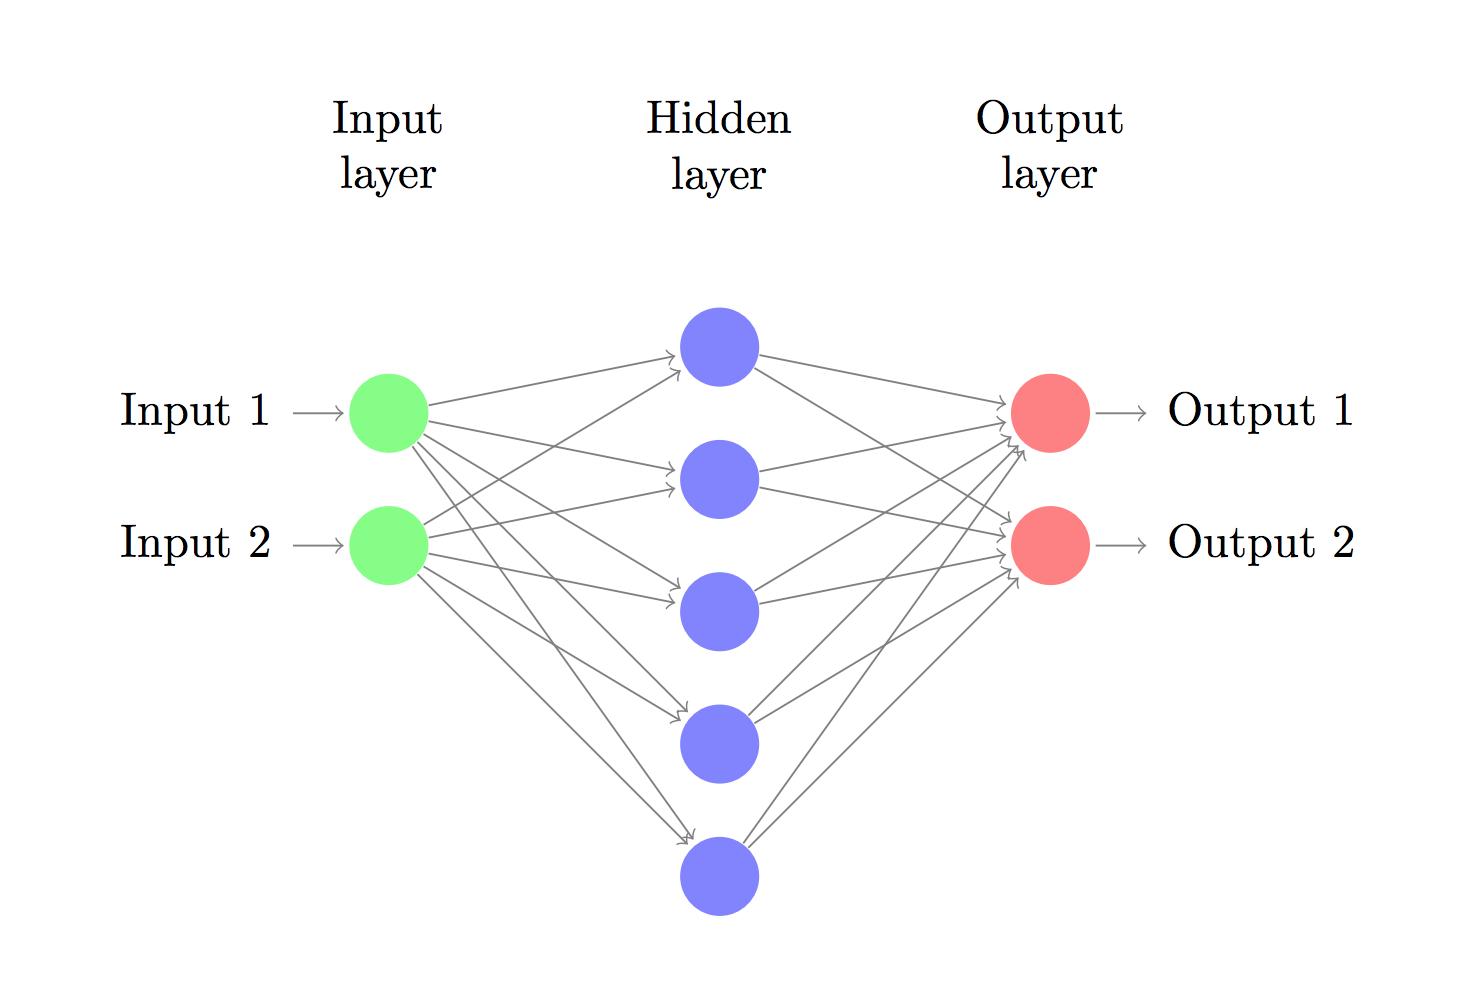
\includegraphics[scale=0.3]{Figures/layers}
	\decoRule
	\caption[Input, Hidden and Output Layers]{Input, Hidden and Output Layers \parencite{DennyBritz2015}}
	\label{fig:layers}
	%https://blog.csdn.net/mydear_11000/article/details/51087980
\end{figure}



\subsubsection{Optimizer Function}

\subsubsection{Supervised vs. Unsupervised Learning}
Supervised learning refers to a task, where a machine learning algorithm learns on data that is labelled. A time series that contains an anomaly that is labelled as such would be an example of such a data set. In contrast, when a machine learning algorithm is applied to an unlabelled data set, it is called unsupervised learning. The goal of unsupervised learning is to find hidden patterns (clusters) in the data set.


\section{Background}

Following, it is explained how different kinds of neural networks work and what they are used for.

\subsection{Neural Networks for Anomaly Detection} \label{NN}

Out of the three most popular neural network architectures, convolutional neural networks (CNN), recurrent neural networks (RNN) and deep neural networks (DNN), RNNs are typically used for anomaly detection in time series [e.g \parencite{Malhotra2015}, \parencite{Verner}]. RNNs have built-in memory and are therefore able to anticipate the next value in a time series based on current and past data. Classic or vanilla RNNs can theoretically keep track of arbitrary long-term dependencies in input sequences. There, however, is a computational issue: when using back-propagation to train a vanilla RNN, the back-propagated gradients can "vanish" or "explode" due to the computations involved in the process, which use finite-precision numbers. Because Long Short Term Memory (LSTM) units allow gradients to flow unchanged, RNNs using LSTM unit or Gated Recurrent units (GRU) partially solve the vanishing gradient problem and therefore drastically improve accuracy \parencite{Hochreiter1997}.

Specially to mention in this context are LSTM (Long-Short Term Memory) and GRU (Gated Recurrent Units). Both achieved outstanding performance when used for tasks such as unsegmented, connected handwriting recognition, speech recognition and anomaly detection in network traffic or IDSs (intrusion detection systems) \parencite{JunyoungChung2014}

\subsubsection{LSTM} \label{LSTM}
LSTM was first proposed in 1997 by Schmidhuber and Hochreiter \parencite{Hochreiter1997}. The initial version to the LSTM unit consisted of a cells, input and output gates. In 1999, the LSTM architecture was improved by introducing a forget gate and therefore allowing the LSTM to reset its own state \parencite{Gers2000}. LSTM is used in a supervised training approach, that means it tries to predict a predefined state taking the past and the current state. If the predicted state differs from the expected state, the weights of the different gates are adjusted using an optimizer algorithm such as gradient descent. Figure \ref{fig:LSTM} shows how the gates and the cell are arranged. The cell represents the memory of the LSTM. In simple words, the LSTM works as follows to predict a new value: 

\begin{enumerate}
	\item Forget Gate: Obsolete information is removed from the cell state.
	\item Input Gate: New information is added to the cell state
	\item Output Gate: The new information and the cell state are added to make the new prediction.
	\item The new cell state is propagated to the next LSTM unit  
\end{enumerate}
     
\begin{figure}[h]
	\centering
	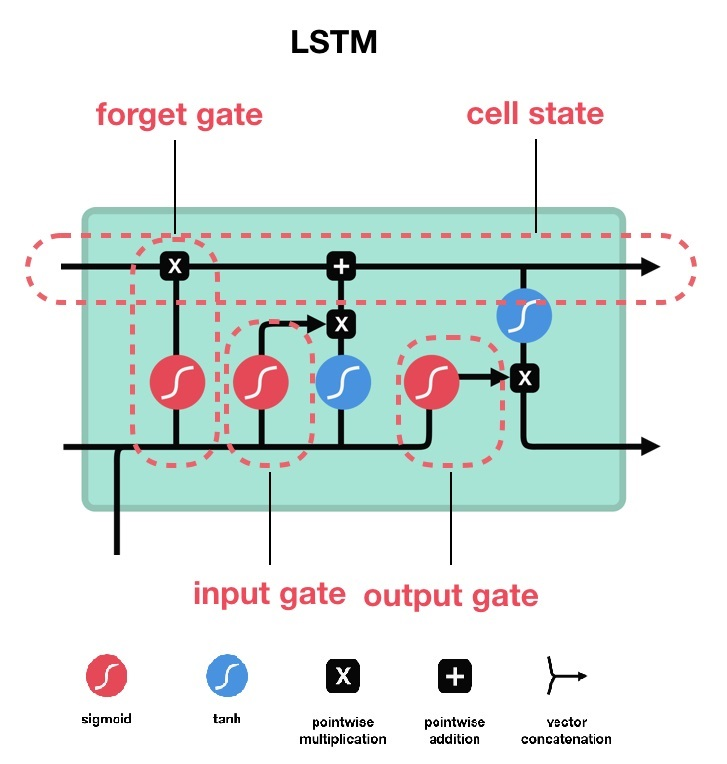
\includegraphics[scale=0.5]{Figures/LSTM}
	\decoRule
	\caption[Gates and Cell of LSTM]{Gates and Cell of LSTM  \parencite{MichaelPhi2018}}
	\label{fig:LSTM}
\end{figure}

% from https://towardsdatascience.com/illustrated-guide-to-lstms-and-gru-s-a-step-by-step-explanation-44e9eb85bf21

%\subsubsection{GRU}
% maybe not necessary

\subsubsection{CNN}
In contrast to RNNs Convolutional Neural Networks are generally used for image classification. CNNs work as feature extractors and are able to recognize patterns . CNNs use layers that are not fully connected, to reduce complexity (compare to \ref{NN}). In a CNN, a set number of neurons forms a filter. These filters or kernels are the actual feature extractors. A filter may represent a line or pattern (see Figure \ref{fig:filter}) \parencite{LeCun1998}.

\begin{figure}[h]
	\centering
	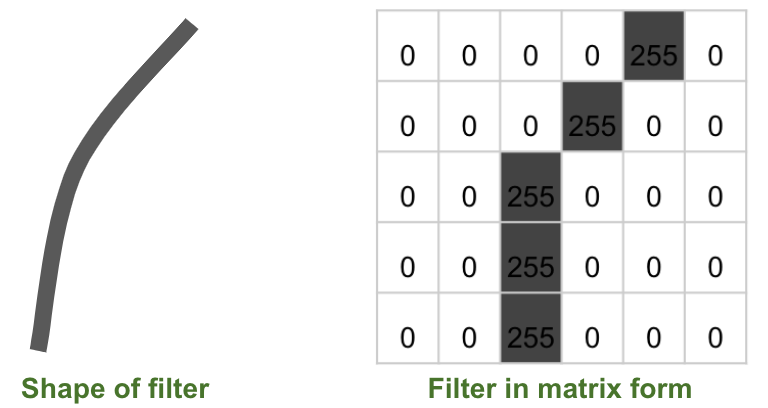
\includegraphics[scale=0.7]{Figures/filter}
	\decoRule
	\caption[Example of a Filter used in CNN]{Example of a Filter used in CNN \parencite{RichStureborg2019}}
	\label{fig:filter}
\end{figure}

To detect whether, a feature is occurrent in a picture, the filter is gradually moved over the picture in so called strides. In every step (stride) the dot-product between the filter and the part of the picture is calculated. The results of the operations are stored in activation maps.  The greater the dot-product the more alike are the filter and the section of the image. Training the network hereby refers to determining the shapes of these filters.
Other typical features of a CNN are the pooling layers. The pooling layers reduce the amount of computation necessary. The most commonly used pooling technique is max-pooling and works as shown in Figure \ref{fig:pooling}.

\begin{figure}[h]
	\centering
	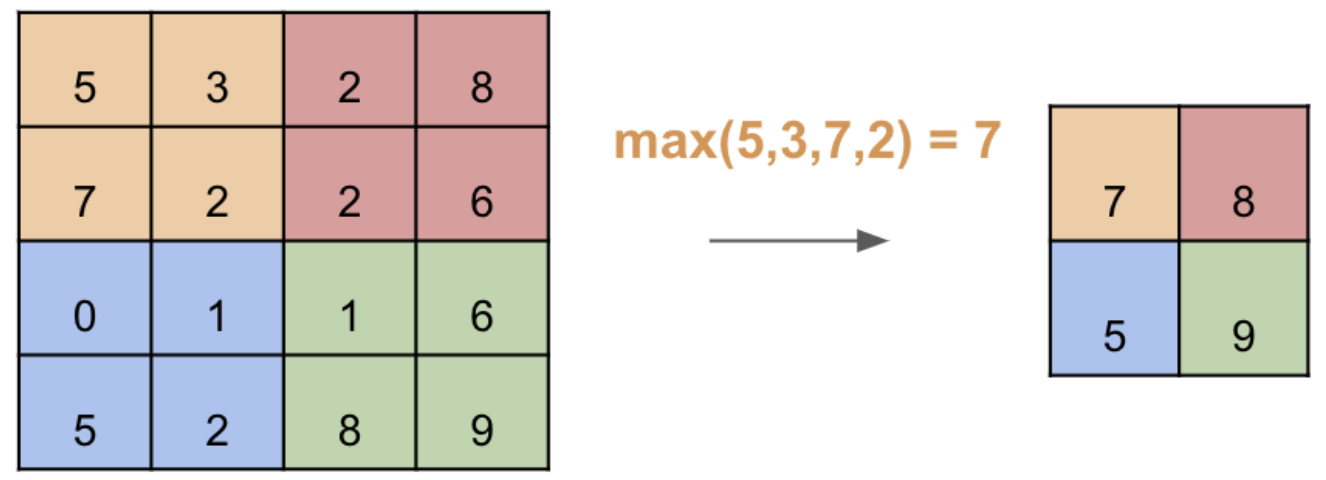
\includegraphics[scale=0.2]{Figures/pooling}
	\decoRule
	\caption[Example of max-pooling]{Example of max-pooling \parencite{RichStureborg2019}}
	\label{fig:pooling}
\end{figure}

The idea of max-pooling is to only keep the maximum value of an activation map. In the orange region 7 represents the maximum value, so it is kept while the other values are discarded \parencite{RichStureborg2019}.

In 2019, Wen and Keys proposed to use CNN also for anomaly detection in time series since it shares many common aspects with image segmentation. A univariate time series is therefore viewed as a one-dimensional image.\\ 


% https://towardsdatascience.com/conv-nets-for-dummies-a-bottom-up-approach-c1b754fb14d6


\subsection{Transfer Learning}
%https://builtin.com/data-science/transfer-learning
%Section about transfer learning\\
The reuse of a previously trained model on a new problem is known as transfer learning. It is currently very popular in deep learning because it can train deep neural networks with a relatively small amount of data. This is particularly useful in the field of data science, as most real-world problems do not provide millions of labeled data points to train complex models.
In transfer learning, the knowledge of an already trained machine learning model is applied to a different but related problem. For example, if a classifier was trained to predict if an image contains a backpack, the model's experience could be applied to recognize other objects such as sunglasses \parencite{NiklasDonges2020}.

\section{Problem Statement}

Defining a ground truth is one of the most difficult aspects of time series anomaly detection. Determining when anomalous behavior begins and ends in time series is a difficult task, as even human experts are likely to disagree in their assessments. Furthermore, there is the question of what constitutes a useful detection when detecting anomalies in time series.
In the past, RNN have successfully been used for anomaly detection (e.g. [\parencite{Malhotra2015}; \parencite{Fan2016}]. Therefore, designs for various use cases are well researched. RNN are well suited for the task, however, take a long time to train due to the complexity of how a single unit is designed (see \ref{LSTM}). In comparison CNN are not as complex and therefore, generally take less time to train. However, CNNs are generally used for image recognition and were only very recently used for anomaly detection in time series. It is therefore mostly unknown what designs are applicable for successful anomaly detection in time series data. %is this true?
While RNN are able to deal with multivariate data by design, a classical CNN requires design changes to be able to deal with multivariate data. Wen and Keys \parencite*{Wen2019} proposed to use a special kind of U-net, an improved version of a Fully Convolutional Neural Network \parencite{Ronneberger2015}.
Further, a CNN is not capable to analyze streaming data so it relies on segmentation of the data. These data segments are called snapshots. In order to not miss any data points, the frequency of taking these snapshots should be at least as high as the length of snapshot so that every time point is evaluated by the model at least once. However, for better performance it might prove beneficial to use a higher frequency which means every point is evaluated various times by the model \parencite{Wen2019}. The proposed design change and the fact that every point is evaluated multiple times, increases complexity and evaluation time and therefore counteract the architectural advantage of CNN compared to a RNN. 
When designing a neural network many parameters have to be chosen, this applies to both mentioned types of Neural Networks. For example, when designing a CNN, the number of layers, the activation function(s) of a single neuron and the optimizer function have to be chosen. Additionally, when using CNN for time series data the length and frequency of the snapshots have to be determined. Similarly, when designing a RNN also the number of layers and the optimizer function have to be determined. Because the basic building blocks of both networks types are very different it is difficult to fairly compare the complexity of two architecture approaches. Another important parameter which applies to both network types is the number of epochs for which the networks are trained. Through the epochs the training time is determined. In order to compare the two types of neural networks, two networks of similar complexity have to be designed. With equal training time the performance of both can be compared and evaluated. A RNN is therefore only set up as benchmark while the main goal of this research project is to clarify whether CNNs are really useful and propose an advantage over RNNs when applied on time series data for anomaly detection.

%transfer learning is missing

\section{Thesis Statement}

Convolutional Neural Networks are superior to Recurrent Neural Networks when looking for anomalies in time series data regarding training time and complexity.

\subsection{Subquestions}

\begin{itemize}
	\item How does a CNN for univariate and multivariate data need to be designed for successful anomaly detection in time series data?
	\item What advantages and disadvantages arise when using a CNN compared to a RNN for anomaly detection in univariate and multivariate time series?
	\item What parameter settings are crucial for a fair performance comparison between RNN and CNN? 
	\item Optional: How does transfer learning affect the performance of CNN compared to RNN in anomaly detection in time series?
\end{itemize}

 
\subsection{Research Objectives}

Following the research objectives of this paper are defined.

%always start with a verb ... to test, to determine

\begin{enumerate}
	\item Determine what design changes a CNN requires to detect anomalies in time series data.
	\item Determine how the CNN should be designed for the comparison with a RNN
	\item State the advantages and disadvantages of the chosen CNN architecture.
	\item Define parameters which allow a fair comparison of CNN and RNN
\end{enumerate}

\subsection{Limitations}

Recently there have been approaches that combine CNN and RNN into a hybrid network for tasks such as handwriting recognition or video-based emotion recognition \parencite{Dutta2018} \parencite{Fan2016}. However, this paper only compares pure CNN and RNN, and does investigate a hybrid approach.

% AUC and ROC not explained
% Test and training not explained 

\subsection{Significance}

Until now, time series data was almost only approached with RNNs. This paper should answer the question whether CNNs propose a valid alternative and even propose some advantages over RNNs. The paper will answer the fundamental question whether research should channel efforts to further investigate CNNs for anomaly detection in time series data or whether no benefits can be discovered and research is better to focus on other areas. 

\subsection{Chapter Overview}


%----------------------------------------------------------------------------------------

% Chapter Template

\chapter{Related Literature} \label{relatedLiterature} % Main chapter title

\label{2.} % Change X to a consecutive number; for referencing this chapter elsewhere, use \ref{ChapterX}

%----------------------------------------------------------------------------------------
%	SECTION 1
%----------------------------------------------------------------------------------------

\section{Anomaly or Outlier?} \label{anomalies}

Generally, there is no agreement on how to distinguish between anomalies and outliers. The following often used citation claims equality of the term outliers and anomalies.\\

\noindent\enquote{\itshape Outliers are also referred to as abnormalities, discordants, deviants, or anomalies in the data mining
	and statistics literature.} - Aggarwal \parencite*{Aggarwal2013}\\

By others, outliers are regarded as corruption in data, while anomalies are abnormal points with a particular pattern. 
In the context of this paper, only the term anomaly is used to refer to such irregular behaviour. It is hereby important to provide a clear definition for the concept of anomaly. This is critical since different meanings of abnormalities necessitate different detection methods. As a result, it is important to identify the key characteristics of anomalies and to use the description to highlight the boundaries. Following, two common definitions of anomalies:\\

\noindent\enquote{\itshape Anomalies are patterns in data that do not conform to a well-defined notion of normal behaviour.} - Chandola et al. \parencite*{Chandola2009}\\

Ord \parencite*{Ord1996}, defines anomalies as follows:\\

\noindent\enquote{\itshape An observation (or subset of observations) which appears to be inconsistent with the remainder of that set of data.}\\

Anomalies have two major features, according to both definitions:

\begin{itemize}
	\item The anomalies' distribution deviates significantly from the data's overall distribution.
	\item Standard data points make up the vast majority of the dataset. The anomalies make up a very small portion of the overall dataset.
\end{itemize}

The development of anomaly detection methods is dependent on these two factors. The second property prevents the employment of common classification methods that depend on balanced datasets.

\subsection{Types of Anomalies}
Anomalies come in a variety of shapes and sizes. Braei and Wagner \parencite*{Braei2020}  divide the anomalies into three categories:

\begin{enumerate}
	\item \textbf{Point Anomalies} - A point anomaly occurs when a single point deviates dramatically from the rest of the data.
	A point anomaly in a time series is, for example, a temperature peak in an otherwise, over time, steady temperature.
	\item \textbf{Collective Anomalies} - Individual points may or may not be anomalous, but a series of points may be. A time series example could look as follows: A bank customer withdraws \$500 from her account per weekday. Although withdrawing \$500 every now and then is common for the consumer, a series of withdrawals is unusual.
	\item \textbf{Contextual Anomalies} - Some points can appear natural in one context but be identified as anomalous in another: In Germany, a daily temperature of 35 degrees Celsius is considered natural in the summer, but the same temperature in the winter is considered unusual.
\end{enumerate}

Knowing ahead of time what kind of anomaly the data might contain helps the data analyst choose the best detection process. Some methods for detecting point anomalies fail to detect collective or contextual anomalies entirely \parencite{Braei2020}. 

%\subsection{Time Series Patterns}
%
%There are a few key characteristics of time-series that are briefly described here.
%
%\subsubsection{Level}
%
%The mean of the series is used to determine the time-series standard. When a time-series has a pattern, the level is also said to be changing.
%
%\subsubsection{Trend}
%
%If the mean of a time series does not remain constant over time but increases or decreases, it is said to have a trend. A pattern can be either linear or non-linear in nature. Figure 3 shows a positive trend from 2005 to 2008, and then a downward trend after that.
%
%\begin{figure}[h]
%	\centering
%	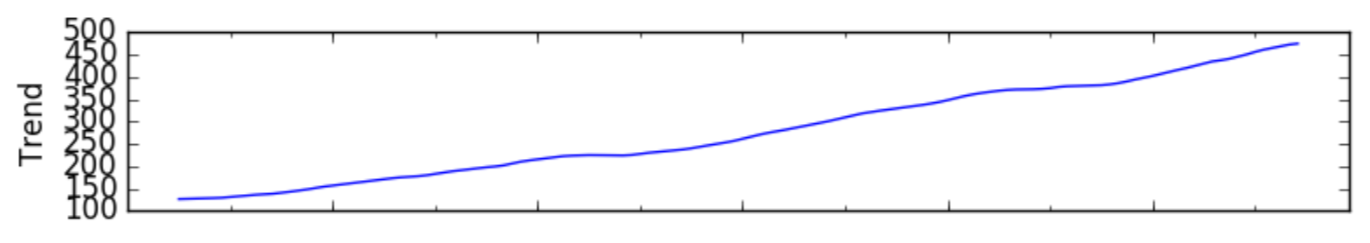
\includegraphics[scale=0.3]{Figures/Trend}
%	\decoRule
%	\caption[Trend]{Trend \parencite{}}
%	\label{fig:Trend}
%	%https://medium.com/swlh/time-series-analysis-7006ea1c3326
%\end{figure}
%
%\subsubsection{Seasonality}
%
%Seasonality refers to the occurrence of variations on a regular basis. Seasonal variables such as the time of year, day of the week, and other similarities influence the time-series, which is why it is called seasonal. As a result, it has a set period of time that is often limited to a year. A seasonal time-series is depicted in Figure 4 \parencite{Braei2020}.
%
%\begin{figure}[h]
%	\centering
%	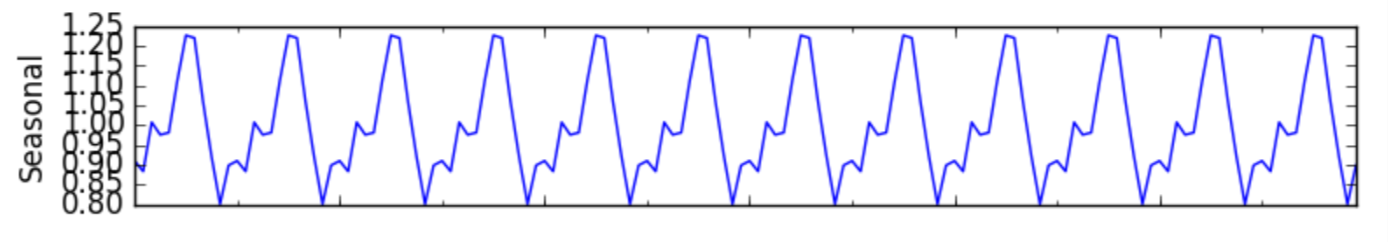
\includegraphics[scale=0.3]{Figures/Seasonal}
%	\decoRule
%	\caption[Seasonality]{Seasonality \parencite{}}
%	\label{fig:Seasonality}
%	%https://medium.com/swlh/time-series-analysis-7006ea1c3326
%\end{figure}
%
%\subsubsection{Noise}
%
%The variability in the observations that the model cannot account for.
%
%\begin{figure}[h]
%	\centering
%	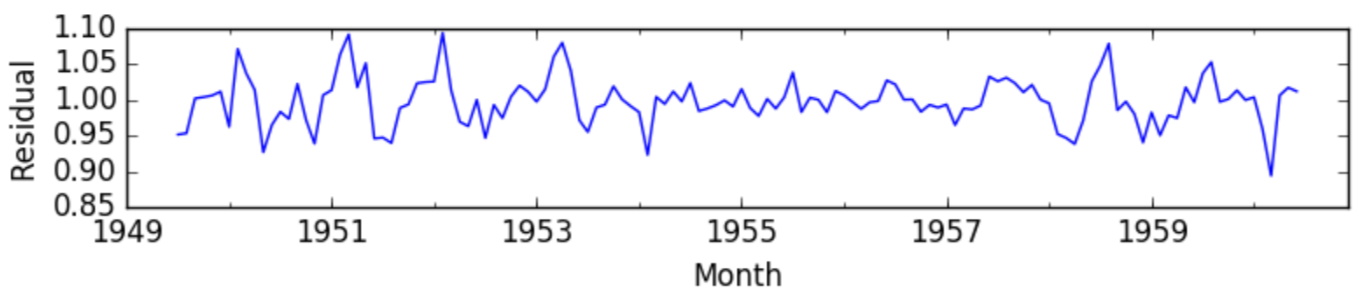
\includegraphics[scale=0.3]{Figures/Residual}
%	\decoRule
%	\caption[Noise]{Noise \parencite{}}
%	\label{fig:Noise}
%	%https://medium.com/swlh/time-series-analysis-7006ea1c3326
%\end{figure}
%
%\subsubsection{Observed}
%
%All the above componenents combined could provide the observed time series shown in Figure . The components may add up to form a model such as: 
%
%\begin{equation}
%	Y =level + trend + seasonality + noise
%\end{equation}
%
%\begin{figure}[h]
%	\centering
%	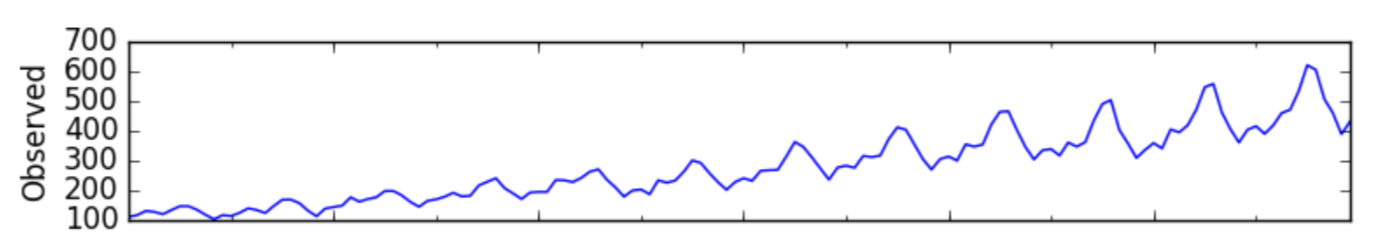
\includegraphics[scale=0.3]{Figures/Observed}
%	\decoRule
%	\caption[Observed]{Observed \parencite{}}
%	\label{fig:Observed}
%	%https://medium.com/swlh/time-series-analysis-7006ea1c3326
%\end{figure}

\section{Anomaly Detection on Univariate Time Series} \label{Anomaly Detection on Univariate Time Series}

First, anomaly detection on univariate time series using deep learning approaches is investigated to gain insight into the used architecture and the overall training and detection process. 

\subsection{Univariate Anomaly detection with LSTM}

Because of their ability to retain long term memory, Long Short Term Memory (LSTM) networks have been shown to be especially useful for learning sequences containing longer term patterns. Malhotra et al. \parencite*{Malhotra2015} model normal behaviour with a predictor and then use the prediction errors to classify abnormal behaviour. This is especially useful in real-world anomaly detection scenarios where instances of normal behaviour are plentiful, but instances of anomalous behaviour are rare. For prediction, multiple time steps into the future are forecasted to ensure that the networks capture the temporal structure of the chain. As a result, each point in the series has multiple corresponding expected values made at various points in the past, resulting in multiple error values. The likelihood of normal behaviour on the test data is calculated using the probability distribution of the errors produced when predicting on normal data. For this approach Malhotra et al. \parencite{Malhotra2015} use a deep LSTM neural networks. The proposed network architecture with two hidden layers is successfully applied on different univariate time series such Electrocardiograms (ECG), a valve time series and a power demand dataset. The proposed approach on univariate data could easily be adopted with multivariate data, where instead of a univariate in- and output, a multivariate data set is fed into the neural network to predict a multivariate output. 

Malhotra et. al \parencite*{Malhotra2015} use an interesting split of the dataset to train the neural networks. The data was divided into four sets. a non-anomalous training set, a non-anomalous validation set, a mixture of anomalous and non-anomalous validation set and test set, also consisting of an anomalous and non-anomalous sequences. This approach was chosen to deal with the rare class problem, which is typical in anomaly detection. Since non-anomalous data is plentiful, the model is trained in an unsupervised fashion, predicting the future, but not able to classify if anomalous behaviour was present. The goal of this approach was to establish a baseline of non-anomalous behaviour with the training set. The learned model was then validated and tested with anomalous and non-anomalous data to evaluate its performance.

%https://www.elen.ucl.ac.be/Proceedings/esann/esannpdf/es2015-56.pdf


\subsection{Univariate Anomaly detection with CNN} \label{CNN on univariate series}

The use of CNNs for time-series analysis has received interest in recent years. Munir et al. \parencite*{Munir2019} forecast time-series and identify anomalies based on the prediction error using a CNN architecture called deep-learning based anomaly detection method (DeepAnT). DeepAnT uses an architecture that is divided into two modules. The first module is called "Time Series Predictor". The "Time Series Predictor" consists of a CNN. As the name of the module indicates, the CNN is responsible for predicting the future time stamps of a given time series, whereas  the "Anomaly Detector" module is responsible for tagging given data point as anomalous. Figure \ref{fig:CNN} represents the architecture of the CNN-based predictor module. It consists of two convolutional layers, each followed by a max-pooling layer. As the last layer, however, a fully connected layer, where all neurons are connected to all neurons of the previous layer, is used. The last is responsible for predicting the next time step. The number of output nodes, hereby, corresponds to the number of predicted time steps. One output node means only the next time step into the future is predicted, whereas three output nodes would imply a sequence of three data points are predicted.     


\begin{figure}[h]
	\centering
	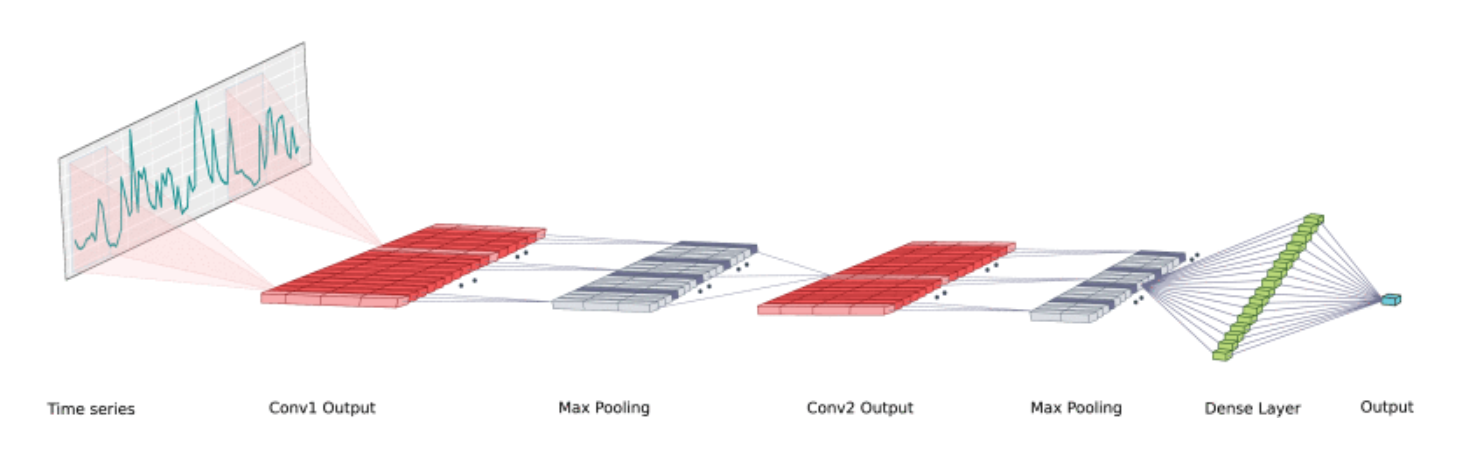
\includegraphics[scale=0.4]{Figures/CNN}
	\decoRule
	\caption[CNN Architecture for Time Series]{CNN Architecture for Time Series \parencite{Munir2019}}
	\label{fig:CNN}
	%https://ieeexplore.ieee.org/document/8581424?denied=
\end{figure}

Once the next time steps are predicted, the values are then passed to the "Anomaly Detector". The detector module calculates the Euclidian distance between the predicted and the actual data point. This measure of discrepancy is used as anomaly score. A high anomaly score indicates a significant anomaly at a given time step. In order to classify the time samples as anomalous and non-anomalous, an anomaly threshold must be specified. The anomaly threshold classifies all data points that lie under the threshold, where the Euclidean distance of predicted and actual value is small, as normal. In contrast all points that exceed the threshold are classified as anomalous. Depending on how low the threshold is set, the sensitivity can be increased \parencite{Munir2019}. In fact, such a threshold is required by all unsupervised anomaly detection algorithms. 

\clearpage
\subsection{Comparison} \label{comparison}
In an extensive study Braei and Wagner \parencite*{Braei2020} compared 20 different anomaly detection methods. The anomaly detection methods were divided into the three following  categories. 

\begin{itemize}
	\item Statistical Methods
	\item Classical Machine Learning Methods
	\item Deep Learning Based Methods (Neural Networks)
\end{itemize}


\subsubsection{Comparison of AUC}
The above stated methods were applied by Braei and Wagner \parencite*{Braei2020} on data containing point, collective and contextual anomalies. In order to compare the different approaches, AUC-Values \footnote{An ROC curve (receiver operating characteristic curve) is a graph showing the performance of a classification model at all classification thresholds. The AUC measures the entire two-dimensional area underneath the entire ROC curve. See section \ref{AUROC}} were used. The results showed that the statistical methods generally performed best on point and collective anomalies while deep learning approaches performed rather poorly. On a dataset that contained contextual anomalies, the situation reflected the exact opposite. Deep learning approaches clearly outperformed statistical methods. It was observed that deep learning approaches kept their ability to generalize while statistical methods overfitted on the data \parencite{Braei2020}.

\subsubsection{Computation Time}
The second parameter that was used to compare the different categories was training and inference time. Inference refers to the time used to classify the test data. Compared to statistical methods and classical machine learning, deep learning approaches once again performed rather poorly regarding training time. Looking at inference time deep learning approaches generally perform well, outperforming the other two categories. However, there are huge difference within the deep learning approaches. While CNNs have a very low inference time, and outperform most other algorithms, LSTMs have the highest inference time of all tested algorithms \parencite{Braei2020}.  


%https://arxiv.org/pdf/2004.00433v1.pdf
\section{Anomaly Detection on Multivariate Time Series}
In this section, anomaly detection on multivariate time series is investigated. Once again, CNNs and LSTMs are examined on the state of the art application possibilities for anomaly detection or time series classification.

\subsection{Multivariate Anomaly Detection with LSTM}
First, relevant works that use LSTMs are investigated. LSTMs will be used to establish a benchmark.

\subsubsection{Supervised Anomaly Detection using LSTM} \label{Anomaly Detection using LSTM}
In his dissertation, Alexander Verner \parencite*{Verner2019}, compared different versions of LSTM Neural Networks against traditional machine learning algorithms such as Support Vector Machines (SVM) and Random Forests. The various algorithms were applied to data of sensors that measure blood glucose levels. To measure the blood glucose levels multiple sensors are used for an accurate result, thus a multivariate time series is the outcome. The data set used in Verner's work did not contain anomalies by default, but the anomalies were embedded into the data set artificially. Since the data was also labelled after the type of anomaly it contained, the learning approach can be classified as supervised. Thus, the goal of the study was to correctly classify which anomaly was present. The first approach used a deep or stacked LSTM, with 10 units in the first layer and 35 in the second. The resulting accuracy of only 0.4 was, however, rather disappointing. This poor performance was explained with an occurring information loss within the deep network. Next, a single layer architecture, with 100 units was proposed. With just a 10\% increase the resulting accuracy was still unacceptable. In a third attempt, the neural network was enriched with an embedding layer. Using this technique, the neural network was able to detect the relationship between the frequencies of measurements that were closely positioned in the time-series. It achieved an accuracy of 98\%. The final architecture proposed by Verner \parencite*{Verner2019} then used bidirectional LSTMs (BLSTMs). According to Graves \parencite*{Graves2005}, BLSTM outperform LSTM on supervised labelling tasks. A BLSTM can extract even more information from raw data by considering the relationship of each measurement to both previous (past) and subsequent (future) measurements in the input time-series. This enhancement resulted in a 99\% accuracy. This impressive accuracy, however, comes at a cost. LSTMs are very time consuming and resource intensive to train. Verner \parencite*{Verner2019} used an Amazon Web Service computing instance with 24 CPUs, 4 GPUs and 128 GB of RAM but the training of an LSTM still took about 10 hours.  
%https://nsuworks.nova.edu/cgi/viewcontent.cgi?article=2075&context=gscis_etd

%\subsubsection{Time Series Forecasting using LSTM}
%LSTMs are normally used to forecast time series such as for example stock prices or air temperature. Following the architecture of a use case applied to a weather time series is described and investigated. The data set contains 14 different variables including air temperature, atmospheric pressure, wind direction etc. The goal in this case is to predict the air temperature as dependent variable. For this puspose a stacked GRU network was used \parencite{Chollet2018}. The above described typical use case of an RNN is relevant because it can be applied in an unsupervised learning approach. Similar as in section \ref{CNN on univariate series}, with a traditional RNN, a base could be learned to predict various time steps in the future. The time Again applying the Euclidean distance, a probability for an occurring anomaly could be calculated.
%
%
%
%
%
%
%In a first approach, a neural network using Gated Recurrent Units was proposed, in order to keep the required computation effort low. The used NN had 32 GRUs and one linear neuron in the output layer. This simple architecture was already able to outperform the established baseline, which used only used todays temperature to predict the same temperature for the next day. Since the model seemed to underfit, in a second attempt another layer with GRUs was added, to increase network capacity. The second layer was able to improve the results although not significantly. Since, the network does still not overfit the complexity could be further increased at the cost of computation time. However, a different approach was chosen. Similar as in section \ref{Anomaly Detection using LSTM} a bidirectional approach was considered. The data was therefore reversed and thus processed in antichronological order using the same network architecture as in the previous attempt. The result strongly underperformed, the established baseline indicating that a bidirectional approach would not be able to improve the results achieved with a one-directional approach. For the chosen example, it is important that data is processed in chronological order
%
%
% \parencite{Chollet2018}. 
%
%The above described typical use case of an LSTM is relevant because it can be applied in an unsupervised learning approach. Similar as in section \ref{CNN on univariate series}, with a traditional LSTM a base could be learned to predict various time steps in the future. Again applying the Euclidean distance, a probability for an occurring anomaly could be calculated.

\subsection{Multivariate Anomaly Detection with CNN}
In this section CNNs for anomaly detection but also for classification of time series are investigated. 

\subsubsection{Classification of Time Series Data using CNN}
In their research project Zheng et al. \parencite*{Zheng2014} tried to beat the state-of-the-art classification algorithm for time series, which is the k-Nearest Neighbour algorithm (k-NN). k-NN has been empirically shown to be extremely difficult to beat. The typical problem of the k-NN algorithm, however, is its computation time. Zheng et al. proposed to use their own developed architecture, which is called Multi-Channel Deep CNN (MC-DCNN). Each channel  hereby represents a CNN with convolutional and pooling layers.
Typically channels in CNN are used to extract features from the different spectra of pictures. A coloured picture for example consists of three channels, red, green and blue. Each channel now works as feature extractor on just one colour.
This feature of CNN is now used in time series classification. Every channel learns features independently using a single dimension of the multivariate time series as input. Another difference to image classification is that multivariate time series classification uses multiple 1D subsequences rather than 2D image pixels as data. Because CNN only learn features, no classification can be done. In order to classify, a CNN architecture is combined with a Multilayer Perceptron (MLP) that uses fully connected layers. Figure \ref{fig:MC-DCNN} shows the just described architecture. On the left, the different channels are shown, where every channel takes on its own univariate time series. With the denoted feature maps and pooling layers, the features of the time series are learned. In the MLP on the right, finally, the classification of the time series is done. 
It is important to note that this architecture does not predict the next time steps in the series but instead a given time series is directly classified. The classification is hereby for example used to classify the physical activity depending on the heartrate and is not used for anomaly detection. In order to use the proposed architecture for anomaly detection however, only the output layer has to be changed. 

\begin{figure}[h]
	\centering
	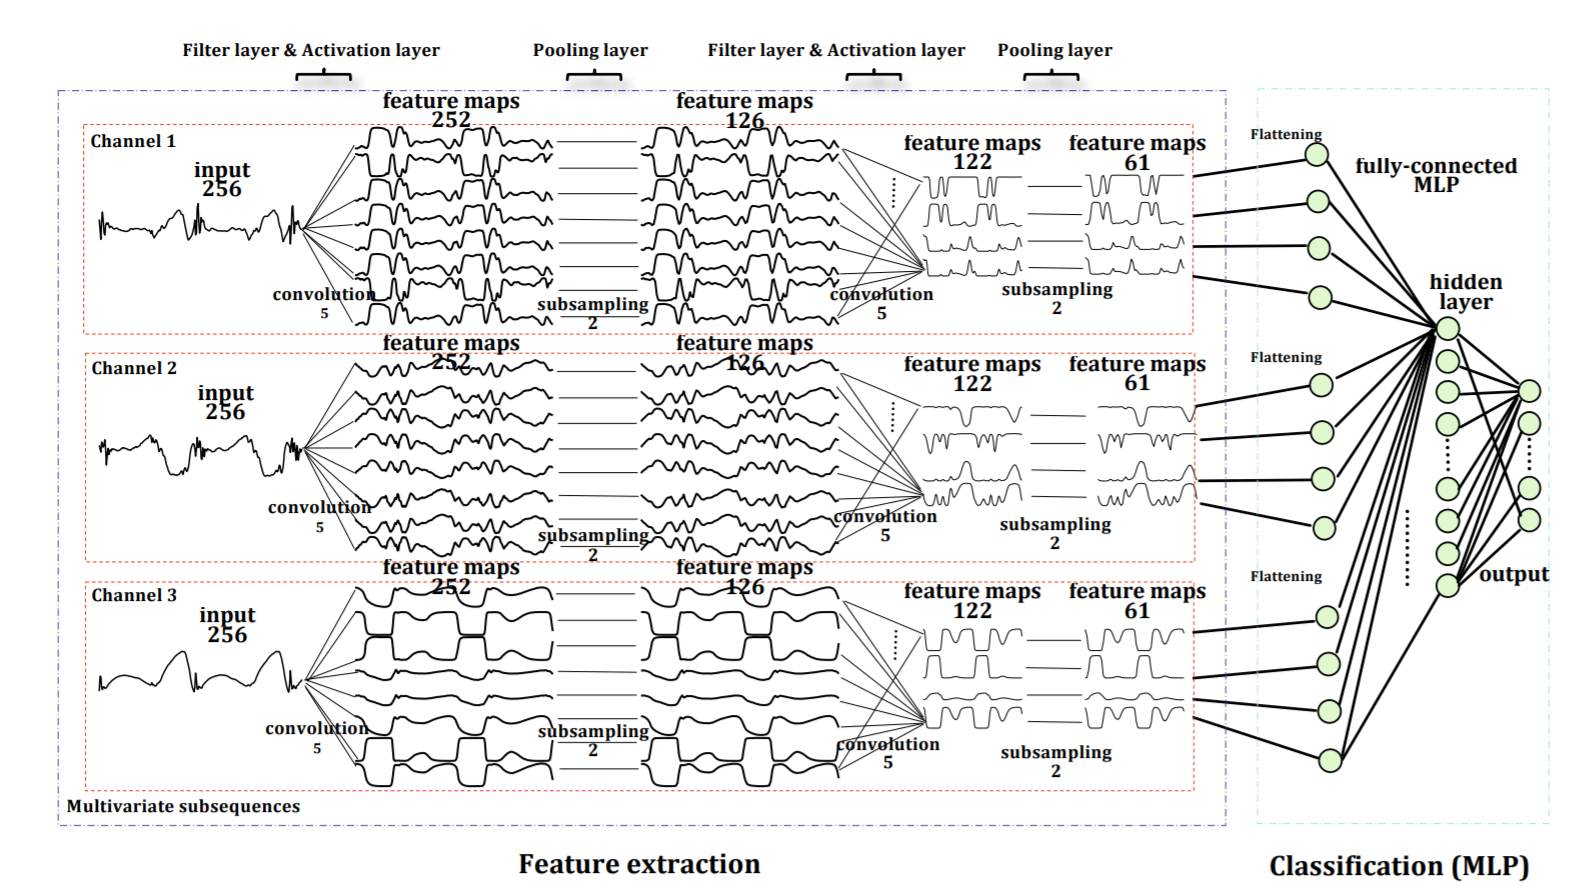
\includegraphics[scale=0.35]{Figures/MC-DCNN}
	\decoRule
	\caption[Architecture of the MC-DCNN]{Architecture of the MC-DCNN \parencite{Zheng2014}}
	\label{fig:MC-DCNN}
	%http://staff.ustc.edu.cn/~cheneh/paper_pdf/2014/Yi-Zheng-WAIM2014.pdf
\end{figure}

Zheng et al. \parencite*{Zheng2014} state that the used architecture was superior to the k-NN algorithm regarding accuracy. Further, the experiments show that deeper architecture are able to learn more robust high-level features. Further, the MC-DCNN architecture performs much faster than the k-NN algorithm, especially when a large dataset is present. The above described architecture could be adopted unchanged in order to classify anomalies.
%http://staff.ustc.edu.cn/~cheneh/paper_pdf/2014/Yi-Zheng-WAIM2014.pdf

\subsubsection{U-Nets for Anomaly Detection} \label{U-Net}
Wen and Keyes \parencite*{Wen2019} use a special type of CNN architecture to detect anomalies. The architecture used is called U-Net. A U-Net consists of so-called encoding and decoding layers. The encoding layers work like a standard CNN whereas the decoding layers are used for upsampling. Upsampling refers to restoring the previously condensed feature maps to its original size. In short, the encoding layers extract the most important features of the time series and decoding layers are using these features to assemble a new time series of the same dimensions as the original one. This encoder-decoder-architecture is often referred to as autoencoder architecture. The main weakness of autoencoders is that in the encoding part through downsampling information is permanently lost. To prevent this information loss, U-Nets introduce so called skip channels also called skip connections. A skip connection, as the name implies, is one that connects an earlier part of the network to a later part of the network and transfers data. The idea is simple: skip channels bring back missing knowledge from some earlier layers so that the network can be properly contextualized. This architecture was proven successful when applied to segmentation of neuronal structures in electron microscopic images in the original paper \parencite{Cicek2016}. In order to handle multivariate time series U-Nets also make use of multiple channels. Figure \ref{fig:U-Net} shows the architecture of the above described U-Net. The left part of the picture shows the encoding layer with five convolutional layers. The encoding layer is followed by the decoding layer, in the right part of the picture. The decoding layer consists of 4 upsampling layers. This symmetric architecture is completed by the yellow lines, that represent the skip channels.

\begin{figure}[h]
	\centering
	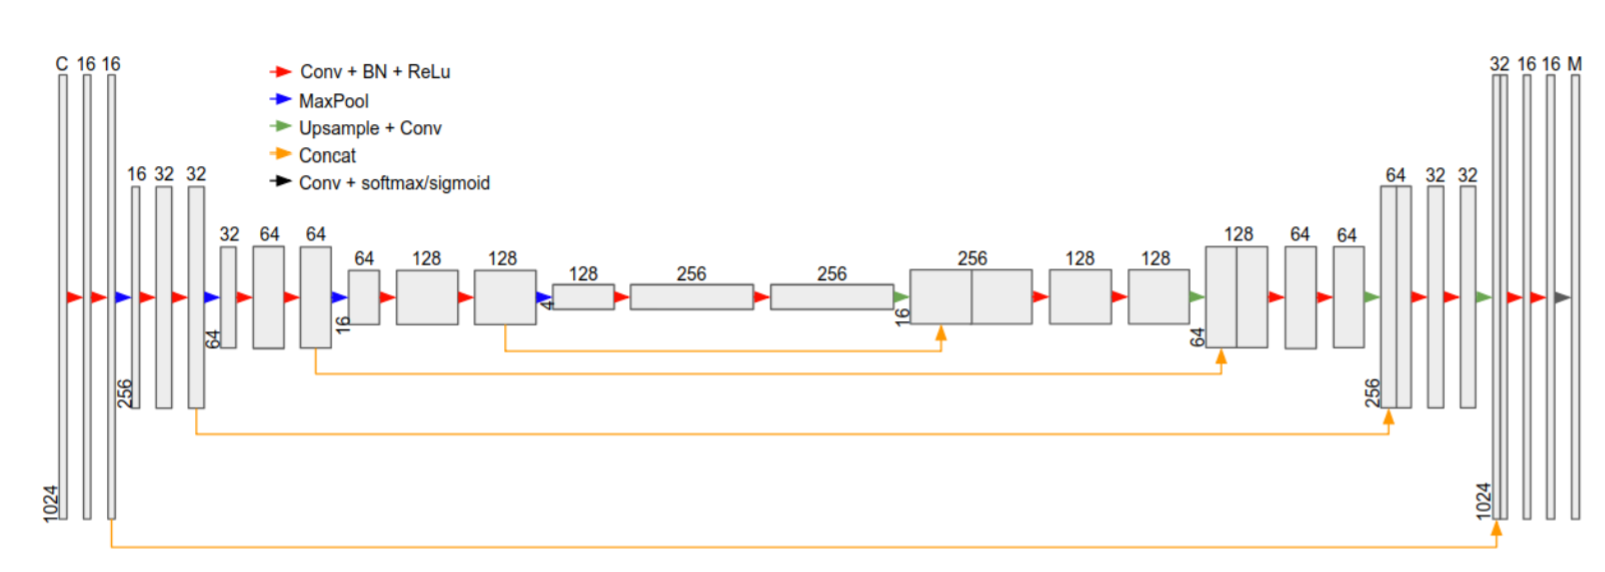
\includegraphics[scale=0.32]{Figures/U-Net}
	\decoRule
	\caption[U-Net Architecture]{U-Net Architecture \parencite{Wen2019}}
	\label{fig:U-Net}
\end{figure}

Finally, the model tries to classify what kind of anomaly the multivariate time series contained e.g a seasonal anomaly (contextual) or a point anomaly. Depending on whether the anomaly classes are mutually exclusive or not either a Sigmoid or Softmax activation is used as last layer activation function.

The proposed U-Net was tested on four scenarios: a univariate task with sufficient data, a multivariate task with sufficient data, a univariate task with insufficient data and transfer learning, and a multivariate task with insufficient data and transfer learning \parencite{Wen2019}. 

For the univariate task the dodgers loop sensor data was used. It involves a 28-week time series of traffic on a ramp near Dodger Stadium with a 5-minute frequency. The goal is to spot unusual traffic patterns caused by sporting events. Out of 39 events, only three could not be detected. The missing detection were attributed to missing values in the data set. Missing values apparently also were the reason for some false positives.

For the multivariate task the gasoil heating loop (GHL) dataset proposed by Filonov et. al \parencite*{Filonov2016} was used. It contains 48 simulated control sequences for a gasoil plant heating loop that was hacked at one stage. There are 19 variables in all time series. A multivariate U-Net with 19 channels was trained by Wen and Keyes \parencite*{Wen2019}. Out the 18, in the test present attacks, only one was missed. However, also 3 false alarms (false positives) were reported. 

%The tasks that included transfer learning are investigated further in Section \ref{TransferLearning}.

%\section{Transfer Learning} \label{Transferlearning}
%The idea behind transfer learning is to transfer knowledge from one domain to another. For example, the knowledge of a Neural Network that classifies pictures of dogs and cats can be used to classify pictures of rabbits. This is possible because all these animals share some features such as eyes or ears. Transfer learning typically uses a neural network that was pretrained on a large dataset. Some layers are then retrained on the target data set, that typically is much smaller and might not consist of enough data to train a powerful Neural Network.
%
%\subsection{Transfer Learning with CNN}
%Since CNN work as feature extractors, the idea when applying transfer learning is to transfer these features to different domains. In the first few layers a CNN typically learns low level features like corners or edges. The features are typically adopted unchanged, meaning the learned weights of the neurons are frozen. The deeper layers of CNN assemble the low level features to high level features such as an ear. Depending on how related the domain of the pretrained and the new network are, deep layers should be retrained to form other features. If a CNN that is trained to recognize animals should be used to classify furniture, the features possibly can not be adopted one-to-one. Instead, the pretrained weights of the neurons are used as initial weights compared to randomly initialised weights when training a CNN from scratch. Using this approach the CNN is fine tuned to new domain using its previous knowledge. The only part of the neural network that is trained from scratch is the classification layer at the end. This part typically consists of the fully connected layers and the output layer. These parts need to adopt to the new classes \parencite{Chollet2018}. 
%
%\subsubsection{Transfer Learning in Anomaly Detection} \label{TransferLearning}
%Wen and Keyes \parencite*{Wen2019} differentiated between transfer learning on univariate and multivariate tasks. For univariate tasks, the architecture, a U-Net, shown in Figure \ref{fig:U-Net} was used. Only the output layer was changed to match the number of classes in the target task. The pretraining was carried out with various data sets containing different kinds of anomalies such as additive outliers, anomalous temporary changes of volatility,
%and violations of cyclic patterns as these are the most common anomalies found in univariate time series. In theory, the features learned on these anomalies should be relevant for general anomaly detection. To pretrain the U-Net, synthetic time series were generated. These time series were enriched with the previously mentioned anomalies to create labelled data set for pretraining. Figure \ref{fig:Pretraing data} shows samples from the pretraining data set. In purple, additive outliers, in green changes of volatility and in red violations of cyclic patterns can be observed.
%
%\begin{figure}[h]
%	\centering
%	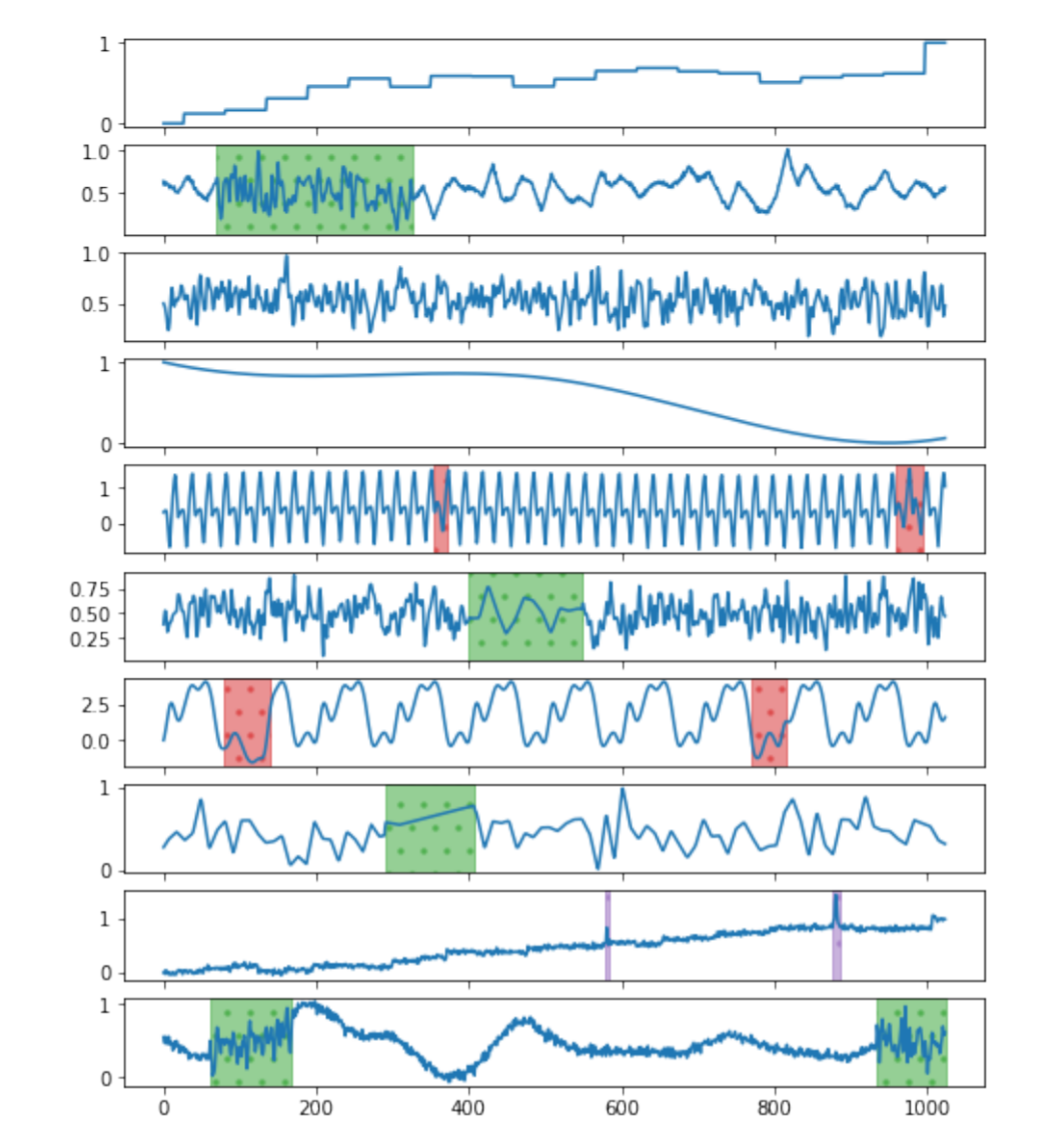
\includegraphics[scale=0.32]{Figures/Synthetic Time Series}
%	\decoRule
%	\caption[Synthetic Time Series]{Synthetic Time Series \parencite{Wen2019}}
%	\label{fig:Pretraing data}
%\end{figure}
%
%\subsection{Transfer Learning with RNN}
%Although not used as often, transfer learning can also be applied when training RNN. Similar to CNN, RNNs require large labelled data sets for training. Therefore transfer learning is valuable approach when a data set is not large enough to train a powerful RNN. When applying transfer learning, RNNs are typically trained on a related source domain, meaning the resulting weights of the neurons figure as a base. The resulting model is then fine tuned on the target domain. When applying transfer learning using RNN, better accuracy and reduced training efforts on the target domain are the main goals \parencite{Gupta2018}.
%
%%https://arxiv.org/pdf/1807.01705.pdf
%
%
%\subsubsection{Transfer Learning for Time Series Analysis}
%Gupta et al. \parencite*{Gupta2018} used a RNN trained on patient phenotypes \footnote{A clinical phenotype is the presentation of a disease in a given individual} to identify previously unseen phenotypes, but also for an unrelated task of in-hospital mortality. The idea was to train a RNN on physiological parameters to classify phenotypes. A phenotype could be the decrease in blood glucose levels. Detecting and classifying a phenotype closely resembles the task of anomaly detection.
%
%To pretrain, Gupta et al. used time series data such as glucose level or heart rate. The goal was to determine, whether a phenotype was present. Since more than one phenotype can be present, the task can be considered as multi-label classification problem. The neural network used consisted of two layers of GRUs. The output layer was designed to represent all possible phenotypes, as activation function the sigmoid function was used. This network was trained on a labelled data set.
%
%The pretrained neural network was then applied to two different target tasks. The target task was slightly reduced in complexity. Instead of a multi-label classification, the problem was formulated as a binary classification problem, determining in case a), whether or not a phenotype was present and in case b) whether a patient would survive, based on the time series observations after Intensive Care Unit (ICU) admission.
%
%
%On the target domain, training with different size data sets was done. The pretrained network was tuned on the target task with at lowest just five percent of data. As a benchmark, to compare the obtained results a logistic regression (LR) and a RNN classifier (RNN-C) were used. The two benchmarks, hereby, only operate on the target domain data set. The performances were compared using AUC (see section \ref{AUROC}) for all used algorithms per data set (Case a \& Case b).   
%
%As expected, the ROC curves of case a) showed that when the training set for the target task is small, the performance gains from transfer learning are greater. Interestingly, in case b) the benchmark RNN is able perform similarly as the two pretrained networks, indicating that better results are obtained the closer related source and target domain are.


\section{Hyperparameter Settings for fair comparison}
In this section it is investigated how CNNs and RNNs can be fairly compared. Since the two's architectures fundamentally differ it is difficult to establish a baseline, where both networks are of similar complexity. In their work Braei and Wagner \parencite*{Braei2020} chose another approach. Instead of trying to build networks with similar complexity, they fine-tuned each evaluated neural network to its full potential and compared their scores as well as their training and inference time. To compare the scores, Braei and Wagner introduced an anomaly threshold (similar as in section \ref{CNN on univariate series}). To find out the optimal threshold, it is varied to optimize sensitivity (true positive rate) and specificity (true negative rate). Varying the threshold and drawing the false positives against the true positives results in the so-called Receiver Operating Characteristics Curve (ROC-Curve), which is used to find the optimal threshold for a certain model. How the ROC-Curve is used to compare different models is explained in the next section.

\subsection{ROC and AUC} \label{AUROC}

The receiver operating characteristic curve, ROC-Curve, and the associated metric area under the curve (AUC), together also called AUROC, which is the area under the ROC-Curve, are two metrics that are frequently used to compare models. This metric is highly useful, especially for detecting anomalies. The ROC-Curve depicts the relationship between the true positive rate and the false positive rate at various threshold values \parencite{Google2021}. The variables needed for the calculations are:

\begin{itemize}
	\item TP: True Positives
	\item FN: False Negatives
	\item FP: False Positives
	\item TN: True Negatives	 
\end{itemize}

	
	The true positive rate is defined as follows: \[TPR = TP/(TP+FN)\]
	
	The false positive rate is defined as: \[FPR = FP/(FP+TN)\]

Typically, lowering the classification threshold, described in section \ref{CNN on univariate series}, causes more items to be classified as positive, which increases both False Positives and True Positives. A typical ROC curve is depicted in Figure \ref{fig:ROC}.

\begin{figure}[h]
	\centering
	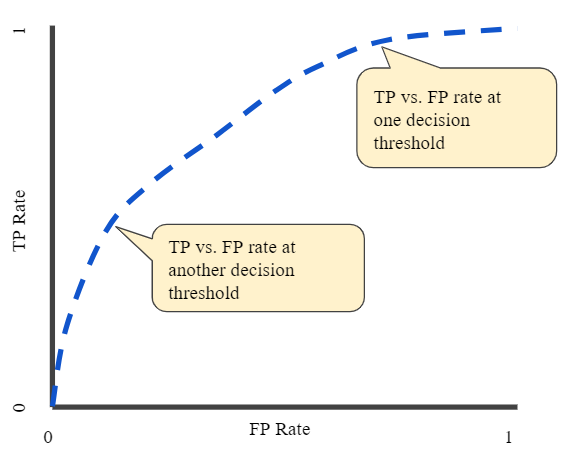
\includegraphics[scale=00.4]{Figures/ROC}
	\decoRule
	\caption[Example ROC-Curve]{Example ROC-Curve \parencite{Google2021}}
	\label{fig:ROC}
	%https://developers.google.com/machine-learning/crash-course/classification/roc-and-auc
\end{figure}

The area under the above shown curve, however, is classification-threshold-invariant. It measures the quality of the model's predictions irrespective of what classification threshold is chosen. The AUC in anomaly detection expresses the likelihood that the measured algorithm assigns a random anomalous point in the time-series a higher anomaly score than a random normal point \parencite{Google2021}. As a result, AUC is considered useful to compare different anomaly detection methods \parencite{Braei2020} .

\subsection{F-Score} 
Another approach to compare models is to use the F-Score. The F-Score describes a model's accuracy on a dataset. It is commonly used to assess binary classification systems, which categorize examples as "positive" or "negative" or in the case of anomaly detection into "anomalous" and "non-anomalous". The F-score is a method of combining the model's precision and recall, per definition it is the harmonic mean of the precision and recall of the model \parencite{Shung2018}. Precision and recall are calculated as follows from the true and false positive respectively negatives.

\[Precision = TP/(FP+TP)\]
\[Recall = TP/(TP+FN)\]

From precision and recall the F-Score, and in this specific case the F1-Score can be calculated as follows.

\[F1 = 2*(Precision*Recall)/(Precision+Recall)\]

When applying the F-Score, a perfect model has a score of 1. Therefore, different models can also easily be compared. In his dissertation, Verner \parencite*{Verner2019}, used the F1-Score to asses different anomaly detection methods.


\subsection{Computation Time}
Another approach to compare the performances is to compare the computation times. To compare the computation times Braei and Wagner \parencite*{Braei2020} looked at the average training and inference time of traditional machine learning models as well as  statistical models and neural networks on univariate time series. Generally, neural networks are expected to invest most of their computation time in training and are able to outperform the traditional machine learning on inference time. However, the practical results showed that Recurrent Neural Networks (LSTM \& GRU) not only needed a long time to train but also had a large inference time on certain data sets. With LSTM performing second best on the given data set, behind k-means clustering, it can be concluded that this comes with a trade-off. On the same data set a CNN was trained. The CNN achieved an AUC-Value of 0.818, compared to 0,84 of the LSTM, which is not much worse than LSTM. Looking at the training and inference time, the CNN is superior. The LSTM takes about 1000 seconds for training and also inference. The CNN, however, trains for 50 seconds, with an inference time of under one second, making the CNN the better choice, when relying on small inference times \parencite{Braei2020}.

\section{Research Gap}
Anomaly detection on time series data has been widely researched. There are comprehensive comparisons of statistical methods, traditional machine learning approaches and neural networks such as the works of Braei and Wagner \parencite*{Braei2020} or Verner \parencite*{Verner2019}. Braei and Wager \parencite*{Braei2020}, focus thereby only on univariate time series. Complementary, Verner \parencite*{Verner2019} only investigated multivariate time series. In their work, Braei and Wagner \parencite*{Braei2020} could show that CNN and RNN are able to achieve similar performances, while CNNs are superior in computation time. Verner \parencite*{Verner2019} faced a similar drawback in his research, where the training of the RNN took approximately 10 hours. 

Since CNNs are only very recently investigated for anomaly detection in time series, Verner \parencite*{Verner2019} did not include them in his research. The approaches presented by Zheng et al. \parencite*{Zheng2014} and Wen and Keyes \parencite*{Wen2019}, however, show promising results, when using CNNs for time series classification respectively anomaly detection. 

As research gap it has been identified that is currently unknown if CNNs are able to outperform RNNs when used in the field of anomaly detection. Braei and Wagner \parencite*{Braei2020} were already able to achieve good results when testing the approach on univariate time series. This work attempts to extend this knowledge to multivariate time series.
%As research gap it has been identified that there is currently no research on how well CNNs perform when used in the field of anomaly detection. The works mentioned above do not establish a state of the art baseline, to compare the achieved results. It is therefore currently not assessable, how useful CNNs are for anomaly detection.

%Further, since the use of neural networks steadily increases, it can be anticipated that transfer learning approaches that save training time, improve accuracy and are able to deal with small data sets will become more popular. Both papers, that compare the different methods for anomaly detection do not take advantage of this approach.

 
%% Chapter 3

\chapter{Research Methodology} % Main chapter title

\section{Introduction}
This section describes which research approach was chosen and why. Further, it elaborates, how the research approach is implemented and what work is done in the corresponding sections. 

\section{Research Design}
As research methodology experimental research was chosen. Experimental research typically focuses on systematically testing a hypothesis. It is often applied to research fields such as physics and chemistry but also psychology. In this research project, the hypothesis to test is formulated as the thesis statement (see section \ref{thesisstatement}).\\
\\
Experimental research knows five process steps. These are:

\begin{itemize}
	\item Awareness of the Problem
	\item Design of Experiments
	\item Experiments
	\item Evaluation
	\item Conclusion
\end{itemize}

In the following, it is outlined what will be done in the different process steps and how it is going to help answering the research question and test the thesis statement. Figure \ref{Thesis Map} illustrates the different steps.

\begin{figure}[h]
	\centering
	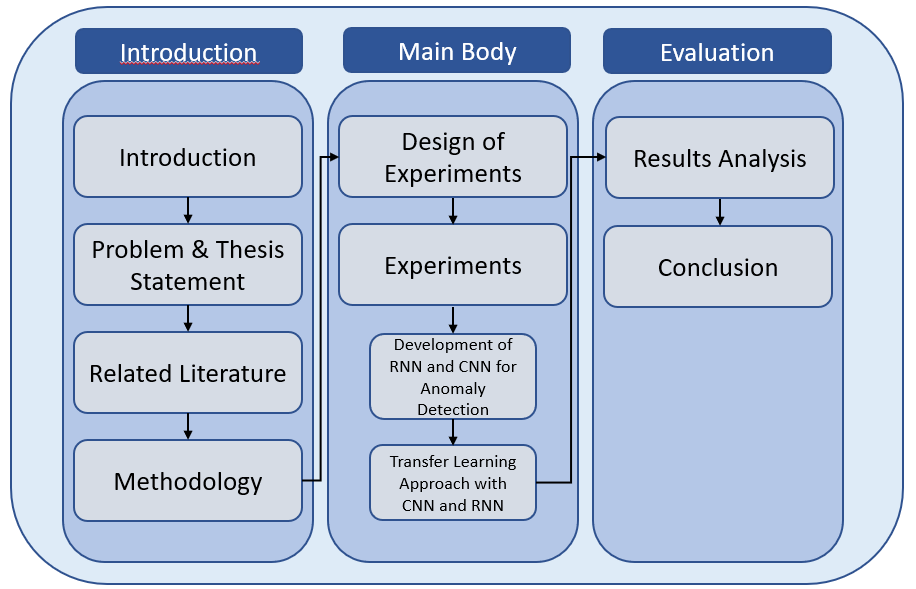
\includegraphics[scale=0.5]{Figures/Thesis Map}
	\decoRule
	\caption[Thesis Map]{Thesis Map \parencite{own}}
	\label{Thesis Map}
\end{figure}

\newpage
\subsection{Awareness of the Problem - Literature Review}
In this work, the literature review consists of two parts, background information presented in Section \ref{background} and the part Related Literature presented as Chapter \ref{relatedLiterature}. The reason for this split is to give insight on how neural networks and especially the derived architectures such as CNN and RNN work. A basic understanding of these two architectures is required to comprehend the problem and thesis statement presented in Sections \ref{Problem} and \ref{thesisstatement}. 

Further, the part Related Literature should deliver insights on how CNN and RNN are applied to detect anomalies. Where helpful, the publications investigated not only focus on detecting anomalies but also on related fields such as classification or prediction of time series. The investigated knowledge fields should serve as suggestions on how anomaly detection models can be set up. 

At last, to be able to answer the research question it is investigated how the different architectures, RNN and CNN, can be compared and what measures are important. 

\subsection{Experimental Design}
In this section, it is outlined how the experiments are designed. It is described how and why datasets are selected as well as which architecture principles are followed when designing the neural networks.

\subsubsection{Data Selection}
As explained in Section \ref{anomalies}, there are several types of anomalies, each of which is more or less difficult to identify. Appropriate data sets are suggested under the Section Experimental Design \ref{ExpDesign}. To perform experiments, at least three separate data sets are suggested. In Section Datasets \ref{Datasets}, it is further reasoned why the proposed datasets are chosen.
 
A careful selection of datasets is critical since it has a direct influence on how experiments must be designed. The datasets define whether a supervised approach may be employed or if only unsupervised methods can be utilized. Because both approaches will be examined, at least one of the datasets must be labeled. 

\subsubsection{Setup of Experiments}
The general setup of the experiments is detailed in the Section Setup of Experiments \ref{SetupOfExperiments}. As discussed in the section Related Literature \ref{relatedLiterature}, there are two basic methods for detecting anomalies: supervised and unsupervised. The Section Section Setup of Experiments \ref{SetupOfExperiments} describes how the neural network topologies must be created for each approach. 
   
Further, in Section \ref{SetupOfExperiments}, all global hyper-parameters are defined. Global hyper-parameters are parameters that must be explicitly defined rather than learnt and are valid across all experiments. The optimizer function and its accompanying parameters are an example of such a global parameter. 

\subsection{Experiments}
Finally, in the Chapter Experiments the proposed experimental setup is implemented. The experiments are only conducted on multivariate time series, since Braei and Wagner \parencite*{Braei2020} already issued a comprehensive study comparing different approaches for anomaly detection on univariate time series. 

In Chapter \ref{Experiments} Experiments, the various experiments are discussed. First, the dataset as well as the contained anomalies are introduced. Following that, the neural network architecture is described, including all hyperparameters that are not globally specified. Finally, the outcomes of the respective experiments are provided. Three experiments with datasets of various complexity are carried out in total.  


\subsection{Evaluation - Results Analysis}
The Chapter Results Analysis is dedicated to the examination of the previously achieved results. The results are compared using predefined metrics such as training time, inference time and F1-Score. Looking at these metrics helps to compare the neural network architectures and to determine whether CNN are actually superior to RNN when applied for anomaly detection. In addtion, insights learned from the experiments are presented and the usefulness of deep learning is ranked.

\subsection{Conclusion}
In the Chapter Conclusion, the research questions are addressed. Answering the research questions will provide an overview of the most significant findings from the experiments. Second, the thesis statement's insights are presented, which aid in determining whether the thesis statement is rejected or accepted. Finally, further research topics are suggested based on the findings of this study. 



%\chapter{Experimental Design}
In this Chapter, the datasets are selected, general design ideas are explained and established, global parameters are defined and at last the experiments and their goals are described.

\section{Tools}
The following Sections provide insight on what tools, such as software and hardware, is used to conduct the experiments.

\subsection{Hardware}
All experiments are conducted on a HP Probook equipped with a Intel Core i7 with 2.8GHz and 32GB of RAM installed. No additional graphics card was used.

\subsection{Software}
All necessary code is written in R (Version 4.1.0). To design the neural networks, the library Keras (Version 2.4.0) together with the Tensorflow (Version 2.5.0) backend is used.


\section{Datasets}
Following, it is motivated how and why the proposed data sets are used.

\subsection{Problems of Existing Benchmarks} \label{Problems of Existing Benchmarks}
In order to find out, which neural network architecture is better suited for anomaly detection, first, suitable datasets have to be evaluated. Most of the papers on anomaly detection test on one of the popular benchmark datasets such as the ones created by Numenta, Yahoo, NASA, or Pei's Lab. These benchmark datasets are, however, declared as flawed by Wu and Keogh \parencite*{Wu2020}. Wu and Keogh state that the benchmark datasets suffer from at least one of the following flaws:

\begin{enumerate}
	\item \textbf{Triviality:} Surprisingly, a sizable proportion of the problems in the benchmark datasets are trivial to solve. Triviality is hereby defined as follows: An anomaly can be found with just one line of code.
	\item \textbf{Unrealistic Density:} This flaw refers to too many anomalies in the dataset or at least in a certain region, whereas in a real world dataset the anomalous data points make up a portion of just above 0 percent.   
	\item \textbf{Mislabeled Ground Truth:} The data in all of the benchmark datasets appears to be mislabeled, with both false positives and false negatives. This is significant for a number of reasons. The majority of anomaly detectors work by computing statistics for each subsequence of some length. They may, however, place their computed label at the beginning, end, or middle of the subsequence. If caution is not exercised, an algorithm may be penalized for reporting a positive just to the left or right of a labeled region.
	\item \textbf{Run-to-failure Bias:} Because many real-world systems are run-to-failure, there is often no data to the right of the last anomaly. Therefore, a naïve algorithm that labels the last point as an anomaly has a very good chance of being correct.
\end{enumerate}

In their work, Wu and Keogh, introduced the UCR Time Series Anomaly Datasets as new benchmark, that avoids the problems listed above. However, at the start of this research project the datasets were not publicly available. Because the search for a dataset, that does not suffer from the above mentioned flaws, would be too time-consuming, the decision was taken to partly engineer own datasets.
\newline
\subsection{Anomalies}
The neural networks should be used to detect various types of anomalies, in order to test their ability to recognize them. Foorthuis \parencite*{Foorthuis2021} compiled, in an extensive literature review, a study on the different types of anomalies. The anomalies were divided into different categories, of which foremost the quantitative multivariate aggregate anomalies are relevant for this research project, especially a) to f) (see figure \ref{fig:Anomaly_types}). These types of anomalies typically occur in time series data, that is composed by sensor data. Examples of such data could be temperature measurements or Electrocardiograms.

\begin{figure}[h]
	\centering
	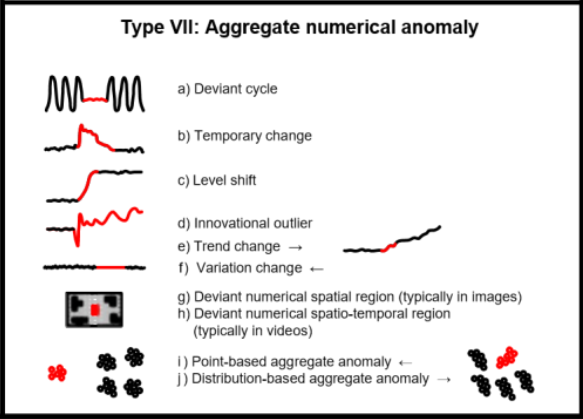
\includegraphics[scale=0.6]{Figures/series_anomaly}
	\decoRule
	\caption[Quantitative Anomalies]{Quantitative Anomalies \parencite{Foorthuis2021}}
	\label{fig:Anomaly_types}
	%https://arxiv.org/ftp/arxiv/papers/2007/2007.15634.pdf
\end{figure}

\subsection{Dataset Selection}
In the following subsections, it is proposed how and why the datasets are selected for the different experiments.

\subsubsection{1. Dataset}
The dataset, which should be used for the first experiment will be of synthetic nature. It consists of various cyclic patterns. In a second step, the dataset is enriched with anomalies. This way, two dataset are produced. The dataset without anomalies is used for an unsupervised learning approach whereas the dataset with labelled anomalies is used for a supervised approach. Further information, on how the dataset is created, what it looks like and what the anomalies look like can be found in Section \ref{dataset1} 

\subsubsection{2. Dataset}
The second dataset, which is used for anomaly detection, should consist of real data. To make sure, that the requirements, mentioned in section \ref{Problems of Existing Benchmarks} are met, the anomalies are embedded manually into the dataset. 

\subsubsection{3. Dataset}
As third dataset, one of the existing benchmark datasets should be used. Despite their obvious flaws, it is still considered useful to validate the previously achieved results on an official benchmark. Further, this gives insights into the overall usefulness of the proposed neural network architectures.

\subsection{Split of Datasets}
With all datasets the classical train, validation and test dataset approach is chosen. For the supervised approach, the training data is enriched with anomalies, whereas for the unsupervised approach a "clean" dataset is used. The final evaluation is done on a test dataset, which is the same for all approaches.


\section{Setup of Experiments} \label{SetupOfExperiments}
The following section explains how the different experiments are conducted in detail. When desinging the experiments, the focus is put on comparability rather than optimally tuned neural networks.  Further, it is shown how the datasets and anomalies were engineered.

The following subsections give information on the chosen setups of the experiments that apply to all experiments. Further, global hyper-parameters are defined. Global hyper-parameters are defined manually and are the same for all experiments. Hyper-parameters, which do not fall in this category such as number of neurons in a layer, are specified in Chapter \ref{Experiments} in the section belonging to the respective experiment.

\subsection{Supervised Learning}
The supervised learning approach refers to training the neural network on a labelled dataset. The dataset used for training already has the anomalies embedded. The task of finding the anomalies can also be described as a classification task, where the neural networks classifies a sequence as normal or anomalous. In such a case binary crossentropy and a sigmoid activation function are used as loss function and last layer activation fuction. The aforementioned combination means that in the last layer a logistic regression is done, where a threshold is determined to classify the sequences into normal and anomalous.

Supervised classification tasks are used and function well when sufficient samples of all classes are available. In anomaly detection, this is generally not the case, as the anomalous is per definition underrepresented. In the literature (e.g. \parencite{Wen2019}), however, the supervised approach is still successfully used. There are two explanation for this: First, as explained in Section \ref{Problems of Existing Benchmarks}, the density of anomalies is unrealistic and second, the anomalies are of the same kind and always look very similar, so a neural network is able to learn the pattern of the anomaly. In the experiments it is investigated, how the neural networks react when presented with anomalies that are similar to the ones in the training data, but also to previously unseen anomalies of the same kind (e.g. level shift). It is expected, that any neural network will fail when there are not enough similar anomalies in the training data.

\subsection{Unsupervised Learning}
The unsupervised learning approach refers to the training of a neural network on a dataset that is free of anomalies. The neural network merely learns the cyclic pattern of the data. When learning the pattern the loss function applied is Mean Absolute Error (MAE), so the learning task is a regression, which itself is supervised. The actual anomaly detection hereby is done in a second step. As proposed in section \ref{CNN on univariate series}, the anomaly detector module, which is also used in this experiment, calculates the Euclidean distance between predicted and actual value, where a large value corresponds to an anomaly.

A unsupervised approach is the more reliable choice when trying to detect anomalies, because the model does not need to know what anomalies might look like. However, setting up this approach is more time consuming, especially when dealing with multivariate time series, as for every variable, a separate detector module and corresponding threshold needs to be set up. It is yet to be expected, that both neural network architectures, CNN and RNN, will outperform their supervised counterparts. 

\subsection{Neural Networks}
The following Sections describe principles that will be used in the design of the neural networks. The described principles and their corresponding paramters are used in all experiments. Parameters that are specific to the experiment are specified in the corresponding section in the Chapter \ref{Experiments}. 

\subsubsection{Normalization}
Before the data is fed into the neural network it is normalized. Normalization ensures that the magnitude of the values that a feature assumes are more or less the same. Therefore, the mean of each time series is subtracted of each time series, and divided by the standard deviation. As normalization parameters, the mean and standard deviation was used for all, test, validation and training dataset.  
%https://towardsdatascience.com/why-data-should-be-normalized-before-training-a-neural-network-c626b7f66c7d

\subsubsection{Activation Function}
When designing the neural networks, as activation function generally "ReLu" (Rectified Linear Unit) is used. The function is non-linear and basically just returns the input if it is bigger than 0 and otherwise 0. This function is widely used, because of its simplicity and generally yields good results with little computation expenses.  

\subsubsection{Optimizer}
As optimizer, the often used default choice in machine learning, ADAM (Adaptive Moment Estimation), with the proposed default values, is applied \parencite{Katanforoosh2019}. ADAM updates the learning rate when training, making it faster than other optimizers such a Gradient Descent. On the downside, however, ADAM uses a lot memory for a given batch size and is found to generalize poorly in late stages of training.
%https://www.deeplearning.ai/ai-notes/optimization/ 

\subsubsection{Batch Computing}
%https://medium.com/analytics-vidhya/when-and-why-are-batches-used-in-machine-learning-acda4eb00763
\textcolor{red}{Typically in machine learning, training examples are not used one after another or all at once, because updating the optimizer function after every example or only after the whole dataset is inefficient as it uses a lot of memory. To speed up the process, training data is fed to the machine learning model in batches. A batch is a collection of training examples. The size of these batches, however, also has an impact on the learning ability of the machine learning model. When using an ADAM optimizer, too large batches can have a negative impact on performance of the model \parencite{Krishnan2019}.\\
When detecting anomlies, the batch size parameter is only used when training. As in a real world scenario every new measurement is analysed immediately since it mostly is crucial to detect the anomaly as early as possible. Analysing every datapoint, however, leads to a increase in computation time which explains the long inference times in the experiments.}
% no batch computing on test sets, because you would not wait for a batch to be complete and just calculate the anomaly score straigth away

\subsection{Experiments}
In the following, it is suggested how the experiments on the 3 different datasets are conducted.

\subsubsection{1. Experiment}
In a first experiment the learning abilities of RNN and CNN are compared. It is investigated how useful the architectures are in a supervised and in an unsupervised setup. This experiment gives general insight on which setups and approaches work under which conditions. As the anomalies embedded are similar in the training and test set, the supervised approaches should yield good results, whereas the unsupervised approaches, given the simplicity of the dataset, are not expected to miss any anomalies.

\subsubsection{2. Experiment}
The second experiment is conducted on a more challenging dataset. Also the embedded anomalies are of a more challenging nature. All approaches that have been found successful in Experiment 1, are investigated further on the new dataset. Since the dataset consists of more, partially dependent, variables, and more challanging cyclic patterns the architectures used in Experiment 1 have to be extended for example by adding additional layers. 

\subsubsection{3. Experiment}
In the third experiment, a dataset that has already been used in the field of anomaly detection should be used. The neural network architecture types CNN and RNN are applied to the chosen dataset. First, this shows which approach is better suited and second, the achieved results can be compared to already existent results to verify the overall performance of the chosen anomaly detection methods.

\subsection{Results}
As results three metrics are reported. First and most important, is the F1-Score which gives insight on the models ability to recognize anomalies.

\textcolor{red}{ F1 Score is picked over AUROC because it's better when the data is imbalanced}

 Second and third, the training and inference time are reported.



  
%\chapter{Experiments} \label{Experiments}
 
\section{Experiment 1}
The first experiment was conducted on a fully synthetic dataset. Supervised and unsupervised learning approaches were used to detect the anomalies. 

\subsection{Dataset} \label{dataset1}
The dataset, that was created for this first task consisted of five variables. The dataset was created under the assumption, that one measurement was drawn per hour on totally 2000 days, resulting in 48000 datapoints. The variables all follow a cyclic pattern shown in Figure \ref{fig:synthetic data} but are not dependent on each other. 

\begin{figure}[h]
	\centering
	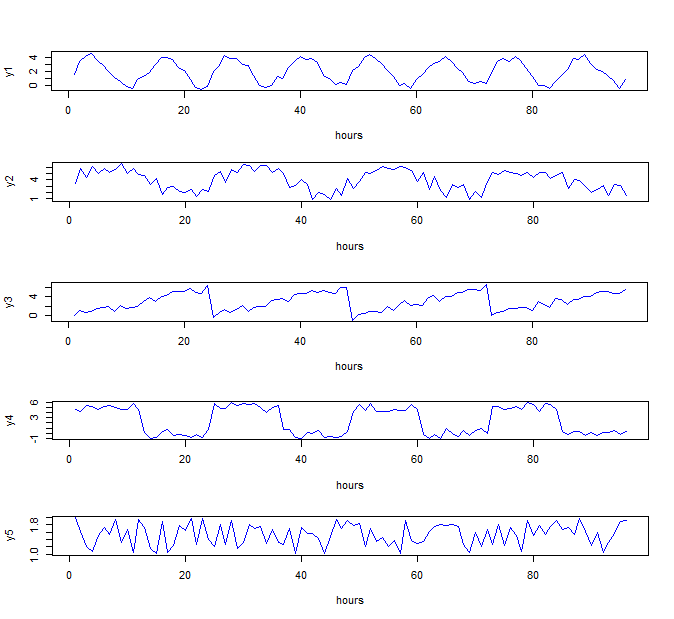
\includegraphics[scale=0.7]{Figures/synthetic data}
	\decoRule
	\caption[Synthetic Dataset]{Synthetic Dataset \parencite{own}}
	\label{fig:synthetic data}
\end{figure}

In a second step the dataset was enriched with six different kinds of anomalies. The anomalies embedded into the dataset are of type deviant cycle, temporary change and level shift. Figure \ref{fig:anomalies} shows examples of the embedded anomalies. The same kind of anomalies were embedded into the training and the test dataset.

\begin{figure}[h]
	\centering
	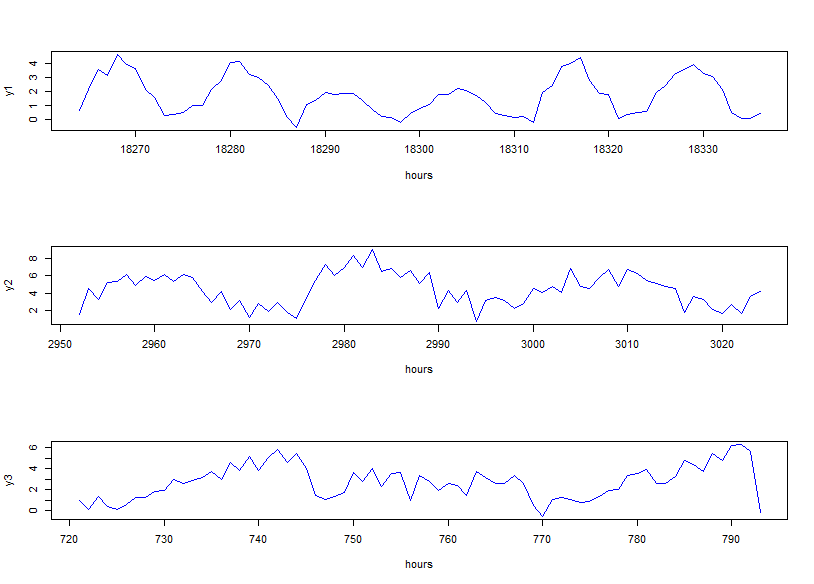
\includegraphics[scale=0.7]{Figures/Anomalies}
	\decoRule
	\caption[Synthetic Anomalies]{Synthetic Anomalies \parencite{own}}
	\label{fig:anomalies}
\end{figure}

For the supervised learning approach the dataset was also labelled. In each case the whole day was marked as an anomaly. In total 30 anomalous days were embedded into the dataset, this corresponds to 1.5 percent of anomalous datapoints.

\subsection{Neural Networks}
In the first experiment, a CNN was tested against a RNN in a supervised and also in an unsupervised fashion. As RNN, the type GRU was chosen. As some first attempts showed, that it showed sufficient results with improved computation time compared to the more complex LSTM. 

For the supervised learning approach, the chosen architecture can be seen in table \ref{Tab:Supervised Learning1}. The architecture with two hidden layers, first presented in Section \ref{Anomaly Detection on Univariate Time Series}, served as example for the RNN. Supplementary, the CNN was built to match the number of layers used for the RNN, where each convolutional layer was followed by a max-pooling layer (explained in Section \ref{CNN}.     

\begin{table}[h]
\caption{Supervised Learning}
	\begin{center}
		\begin{tabular}{ | c | c | c | c |}
			\hline
			\thead{} & \thead{Input} & \thead{NN-Architecture} & \thead{Output} \\
			\hline
			\thead{CNN} &  120 past datapoints  & \makecell{2 1D-Convolutional Layers \\ 2 Max-Pooling Layers \\ 1 Dense Layer}  & \makecell{1 Dense Layer \\ with Sigmoid Activation}   \\
			\hline
			\thead{RNN} &  120 past datapoints  & \makecell{2 GRU Layers \\ 1 Dense Layer}  & \makecell{1 Dense Layer \\ with Sigmoid Activation}  \\
			\hline
		\end{tabular}
		\label{Tab:Supervised Learning1}
	\end{center}
\end{table}

 
The architecture used for the unsupervised learning approach, displayed in table \ref{Tab:Unupervised Learning1}, looked very similar to the architecture of the supervised approach. The main difference between the two architectures was that the CNN was not built as a sequential model, because the used software does not support such an architecture. Instead of having one output layer, the CNN had to be designed with five parallel output layers, each predicting one time series \footnote{More detailed summaries of the models can be found in appendix \ref{AppendixA}}. In comparison, the RNN has just one output layer with 5 neurons, each used to predict a time series.    

\begin{table}[h]
	\caption{Unupervised Learning}
	\begin{center}
		\begin{tabular}{ | c | c | c | c |}
			\hline
			\thead{} & \thead{Input} & \thead{NN-Architecture} & \thead{Output} \\
			\hline
			\thead{CNN} &  120 past datapoints  & \makecell{2 1D-Convolutional Layers \\ 2 Max-Pooling Layers }  & \makecell{ 5 Dense Layers with \\ 1 regression outputs}   \\
			\hline
			\thead{RNN} &  120 past datapoints  & \makecell{2 GRU Layers}  & \makecell{ 1 Dense Layers with \\ 5 regression outputs}  \\
			\hline
		\end{tabular}
	\label{Tab:Unupervised Learning1}
	\end{center}
\end{table}

\subsubsection{Learning}
The learning on the data was done using a so called generator function, which iterates over the dataset in predefined steps. The generator function takes the following parameters:

\begin{itemize}
	\item Lookback - How many data points are considered
	\item Step - How the data is sampled
	\item Delay - How many time steps in the future is the target
	\item Batch Size - The number of samples per batch
\end{itemize}

For this experiment, the parameter lookback was set to 120 data points in the past, which represent the last 5 days. The parameters step and delay were set to one and as batch size 128 was chosen. This setup can be described as follows: There are 128 ordered samples taken from the the whole dataset. Each of these samples consist of 120 data point of past data. With the step parameter set to one, there is not further subsampling done. With delay set to one, the task for the neural network is to predict the next data point in the future per sample for each variable in the data set. This task is done simultaneously for all samples of batch, which speeds up training.

\subsection{Results}

Inference time and F1-Score are, for all models, calculated on the same test dataset. As the initial dataset, it consists of 48000 datapoints, with 30 anomalous days embedded. For the supervised approach using a RNN, no F1-Score is reported, as the model, just like the trivial null classifier, always predicted no anomaly. Since the anomalies span over a whole day, for all approaches, the results were averaged per day. Resulting in normal or anomalous days. The reported F1-Score was finally calculated on this data. 


\begin{table}[h]
	\caption{Results}
	\begin{center}
		\begin{tabular}{ | c | c | c | c |}
			\hline
			\thead{} & \thead{F1-Score} & \thead{Training Time} & \thead{Inference Time} \\
			\hline
			\thead{CNN Supervised} &  0.991388  & 169s  & 422s   \\
			\hline
			\thead{RNN Supervised} &  -  & 967s   & 952s   \\
			\hline
			\thead{CNN Unsupervised} & 0.9989817  & 129s   & 435s   \\
			\hline
			\thead{RNN Unsupervised} &  0.9979613  & 300s   & 793s   \\
			\hline
		\end{tabular}
		\label{Tab:Results1}
	\end{center}
\end{table}

From the table \ref{Tab:Results1}, it can be seen that the supervised learning approach takes longer to train. This can be explained by the fact that a CNN must first learn the patterns and only then begins to recognise the anomalies. \textcolor{red}{Further, it shows that despite promising results when training, the trivial null classifier achieves a higher F1-Score than the supervised CNN approach.}
The best score was achieved with a CNN applied in an unsupervised fashion. The CNN reported just one false negative and a false positive, compared to one false negative and two false positives of the RNN.

\newpage

\section{Experiment 2}
In a second experiment, a real dataset was used as base. The anomalies were embedded manually. Since, the unsupervised approach with RNN in Experiment 1 proved useless it was not included in the second experiment. Since the anomalies in training and test set looked very similar as in Experiment 1, the supervised approach with the CNN was able to recognize some of the anomalies. In the second approach, it should be investigated if this is approach could be of any use, if the anomalies consist of a hitherto unknown pattern.

\subsection{Dataset}
The dataset used was derived from the "Appliances Energy Prediction Dataset" available on the UCI Machine Learning Repository. The dataset consists of 9 room temperatures (T1 to T9) and corresponding humidity levels, energy in use of ligth and appliances, two random variables for testing regression models as well as six variables containing weather information. The dataset consists of 19735 datapoints, where 6 datapoints are drawn per hour. Of the available variables only 10 variables were used for the anomaly detection task. The variables used are 5 room temperatures, energy use, outside temperature, air pressure and wind speed. The variables were selected because they show a dependency. For example, a high outside temperature and energy use result in high temperatures in the different rooms. Figure \ref{fig:temp_dataset} shows an extract from the used dataset.


\begin{figure}[h]
	\centering
	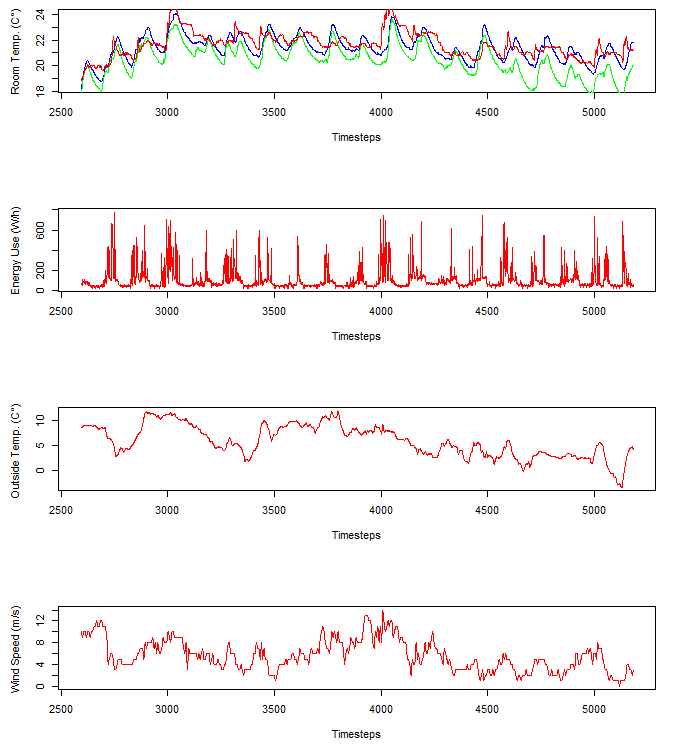
\includegraphics[scale=0.6]{Figures/temp_dataset}
	\decoRule
	\caption[Temperature Dataset]{Appliances Energy Prediction Dataset \parencite{Own or UCI???}}
	\label{fig:temp_dataset}
\end{figure}

\subsubsection{Sampling}
The data set contains datapoints measured between November and May. During this time period, it is observed, that the base temperature steadily rises. This poses the problem, that if the model is trained on data from November to March, with April as validation and May as test period, it is biased on the prevailing colder temperatures. To overcome this problem a special sampling technique was applied. In total six samples of the data set were created. A sample was created by randomly drawing one data point per hour over all datapoints. Four of these sample are then used for training, one for validation and one for testing. Using this sampling technique, the model is no longer biased on certain weather conditions but with the drawback, that the test set is not independent of the test and validation set.   

\subsubsection{Anomalies}
Again, the anomalies were embedded manually into the dataset. The anomalies are of type level shift, deviant cycles, variaton change and distribution-based aggregate anomaly. The anomalies were embedded into the room temperature variables (T1, T2, and T3) and the energy use variable. Figure \ref{fig:temp_anomalies} shows examples of the mentioned anomalies.

\begin{figure}[h]
	\centering
	\includegraphics[scale=0.7]{Figures/temp_anomalies}
	\decoRule
	\caption[Temperature Dataset Anomalies]{Examples of Embedded Anomalies \parencite{Own}}
	\label{fig:temp_anomalies}
\end{figure}

Since the test dataset only consists of around 3000 data points. It was used 3 times so that it does not have an unusual high density of anomalies. In the first instance, anomalies that only affected one variable were embedded. In the second instance, anomalies, that affected all 3 temperature variables, such as a deviant cycle, were embedded. On top, in the energy use variable, variation change anomalies were embedded.  In the third instance, distribution based anomalies, which affected T1 and T2, were embedded.

\subsection{Neural Networks}
Since the RNN did not show sufficient results in Experiment 1 when given a classification task, it was excluded from Experiment 2. The CNN, however, which had probably learned the patterns of the anomalies, was tested again. Since the anomalies in the training and test set are not as similar anymore as in Experiment 1, it is expected that the CNN classifier performs very poorly. 

\begin{table}[h]
	\caption{Unupervised Learning}
	\begin{center}
		\begin{tabular}{ | c | c | c | c |}
			\hline
			\thead{} & \thead{Input} & \thead{NN-Architecture} & \thead{Output} \\
			\hline
			\thead{CNN} &  288 past datapoints  & \makecell{3 1D-Convolutional Layers \\ 1 Max-Pooling Layers }  & \makecell{ 4 Dense Layers with \\ 1 regression outputs}   \\
			\hline
			\thead{RNN} &  288 past datapoints  & \makecell{3 LSTM Layers}  & \makecell{ 1 Dense Layers with \\ 4 regression outputs}  \\
			\hline
		\end{tabular}
		\label{Tab:Unupervised Learning2}
	\end{center}
\end{table}

Because of the complexity of the dataset, in the second experiment it was decided to use LSTM units instead of GRU in the RNN architecture. LSTM units generally provide more accurate results but use more memory and therefore more computation time. The designed neural network architecture consisted of 3 sequential layers of LSTM layers and one dense layer with four neurons. 
%https://analyticsindiamag.com/lstm-vs-gru-in-recurrent-neural-network-a-comparative-study/  

The CNN was designed as follows, three layers of one-dimensional convolutional layers were used. After the first layer, a max-pooling layer was added, to reduce the feature space and improve computation time. Since the CNN is expected to predict a time series, the feature space was not further reduced through max-pooling layers, since it would negatively affect the accuracy.  

\subsubsection{Learning}
The generator function for this experiment was configured as follows:

\begin{itemize}
	\item Lookback - 288 past data points: 12 days in the past
	\item Step - 1: no further subsampling is done
	\item Delay - 1: the next time step in the future is predicted
	\item Batch Size - 128 samples per batch
\end{itemize}

First experiments were done only using data from T1, T2, T3, energy use and outside temperature to predict T1 to T3 and energy use. However as the result were not satisfactory to predict accurate enough results to find the embedded anomalies, further variables were added for training. Finally, the following variables were used to make predictions: T1 to T5, Appliances and Ligths, Outside Temperature, Air Pressure and Windspeed. As the anomlies, however, were only embedded into 4 out of the 10 variables, only the affected 4 were predicted.


\subsection{Results}
Because the dataset was much more challenging, the reported scores are clearly inferior to Experiment 1. In total there were 13 anomalies to be detected in the test sets. The difference in F1-Score between the CNN and the RNN results from one anomaly which was not recognized by the CNN. However, training the RNN takes over 30 times longer than the CNN.

\begin{table}[h]
	\caption{Results}
	\begin{center}
		\begin{tabular}{ | c | c | c | c |}
			\hline
			\thead{} & \thead{F1-Score} & \thead{Training Time} & \thead{Inference Time} \\
			\hline
			\thead{CNN Unsupervised} & 0.666666 & 172s   & 24s*   \\
			\hline
			\thead{RNN Unsupervised} & 0.727272 & 5420s   & 93s*   \\
			\hline
		\end{tabular}
		\label{Tab:Results2}
	\end{center}
\end{table}
* the inference time reported is on just one instance of the test dataset

The above reported results show the overall performance. Since the dataset was more complex than in the first experiment, the results are investigated further to show how the different architecture performed on the various anomalies and how accurate the predictions were on the different variables. First of all, the average error of the predicted variables are investigated further. The below results are reported from the first test set.

\begin{table}[h]
	\caption{Results}
	\begin{center}
		\begin{tabular}{ | c | c | c | c |}
			\hline
			\thead{} & \thead{CNN} & \thead{RNN} \\
			\hline
			\thead{T1} & 0.2712066° C   & 0.1741582° C    \\
			\hline
			\thead{T2} & 0.5236905° C    & 0.9009765° C    \\
			\hline
			\thead{T3} & 0.3210329° C    & 0.7244096° C    \\
			\hline
			\thead{Appliances} & 29.64146 Wh   & 72.91079 Wh   \\
			\hline
		\end{tabular}
		\label{Tab:Average_error}
	\end{center}
\end{table}

From Table \ref{Tab:Average_error}, it can be seen that the CNN outperforms the RNN on all variables except T1. The RNN, however, performs exceptionally well on T1. 
Comparing these results to the performance of the RNN on the first test set shows that only the anomalies that were embedded in T1 are detected. A similar picture emerges in the second test set, since the anomalies affect all 3 variables, a deflection should be visible on all three reported anomaly scores. However, the anomalies detected by the RNN were only visible in the anomaly score reported off T1. While the CNN is not as accurate on any of the variables as the RNN is on T1, this is how the CNN was outperformed. Out off the six anomalies embedded in the second test set, the CNN only recognized one, while the RNN recognized three out of six. On the third test set, both architecture types were able to recognize all anomalies.

Further, as expected, both architecture types were not able to find the variation change anomalies embedded in the variable appliances. The anomaly was constructed as when too many times the exact same value is reported. This anomaly type is with the necessary domain knowledge relatively easy to find.

\section{Experiment 3}
In the third experiment, a dataset that was dedicated to anomaly detection tasks was used. The achieved results can therefore be verified on previously achieved results.

\subsection{Dataset}
%https://arxiv.org/pdf/1612.06676.pdf
The dataset was introduced by Filonov et al. \parencite{Filonov2016}. The data was created by modelling a gasoil plant heating loop The GHL model has three reservoirs: a receiving tank (RT), a heating tank (HT), and a collection tank (CT). The technological challenge is to heat gasoil in RT to 60 degrees Celsius, resulting in a viscosity sufficient for transmission to CT. In the model, the heating is done in stages. A fraction of gasoil is heated to 60 degrees Celsius in HT and then pumped back into RT to relax for a while. This technique is done until the RT temperature reaches 60 degrees Celsius. After that, the RT is poured into the CT. Following that, RT is refilled from an infinite source.

The training dataset consists of 19 variables with no anomalies, the most important, according to Filonov et al. \parencite{Filonov2016} are shown in Figure \ref{fig:GHL_data}. The sensors for RT level, RT temperature, and HT temperature are the first three variables. The remaining two variables relate to control signals for turning on/off the gasoil supply and turning on/off the heater.


\begin{figure}[h]
	\centering
	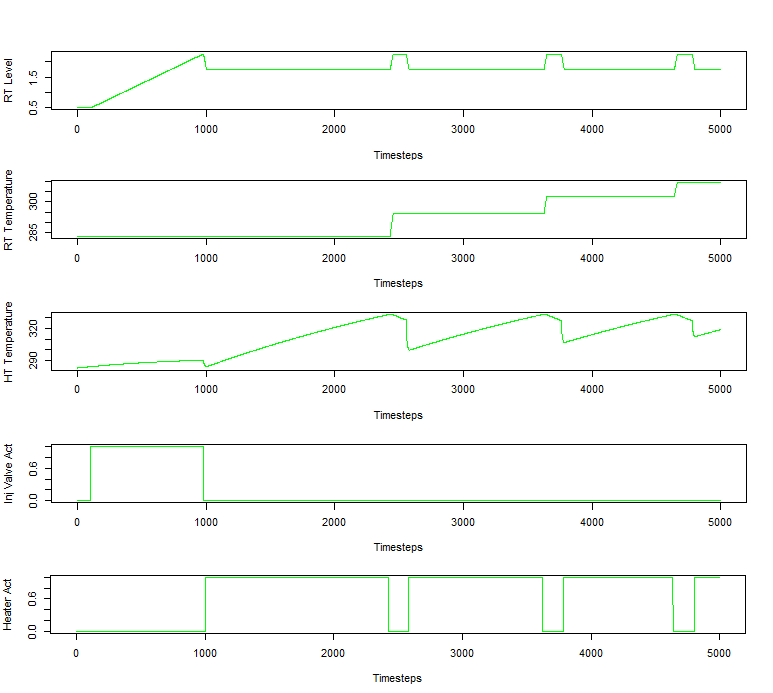
\includegraphics[scale=0.7]{Figures/GHL_data}
	\decoRule
	\caption[Temperature Dataset Anomalies]{Examples of Embedded Anomalies \parencite{Own}}
	\label{fig:GHL_data}
\end{figure}

\subsubsection{Anomalies}
As anomalies cyber attacks were introduced. The anomalies each concern the variable RT Level, which had been changed without authorisation. By setting the value for RT Level to different levels and varying the the time of attack many test sets were created.  

\subsection{Neural Networks}

\subsection{Results}

 

%----------------------------------------------------------------------------------------
%	THESIS CONTENT - APPENDICES
%----------------------------------------------------------------------------------------

\appendix % Cue to tell LaTeX that the following "chapters" are Appendices

% Include the appendices of the thesis as separate files from the Appendices folder
% Uncomment the lines as you write the Appendices

%% Appendix A

\chapter{Model Summaries} % Main appendix title

\label{AppendixA} % For referencing this appendix elsewhere, use \ref{AppendixA}

\section{Summary of Models of Experiment 1}

\subsection{Supervised Learning}
\begin{figure}[h]
	\centering
	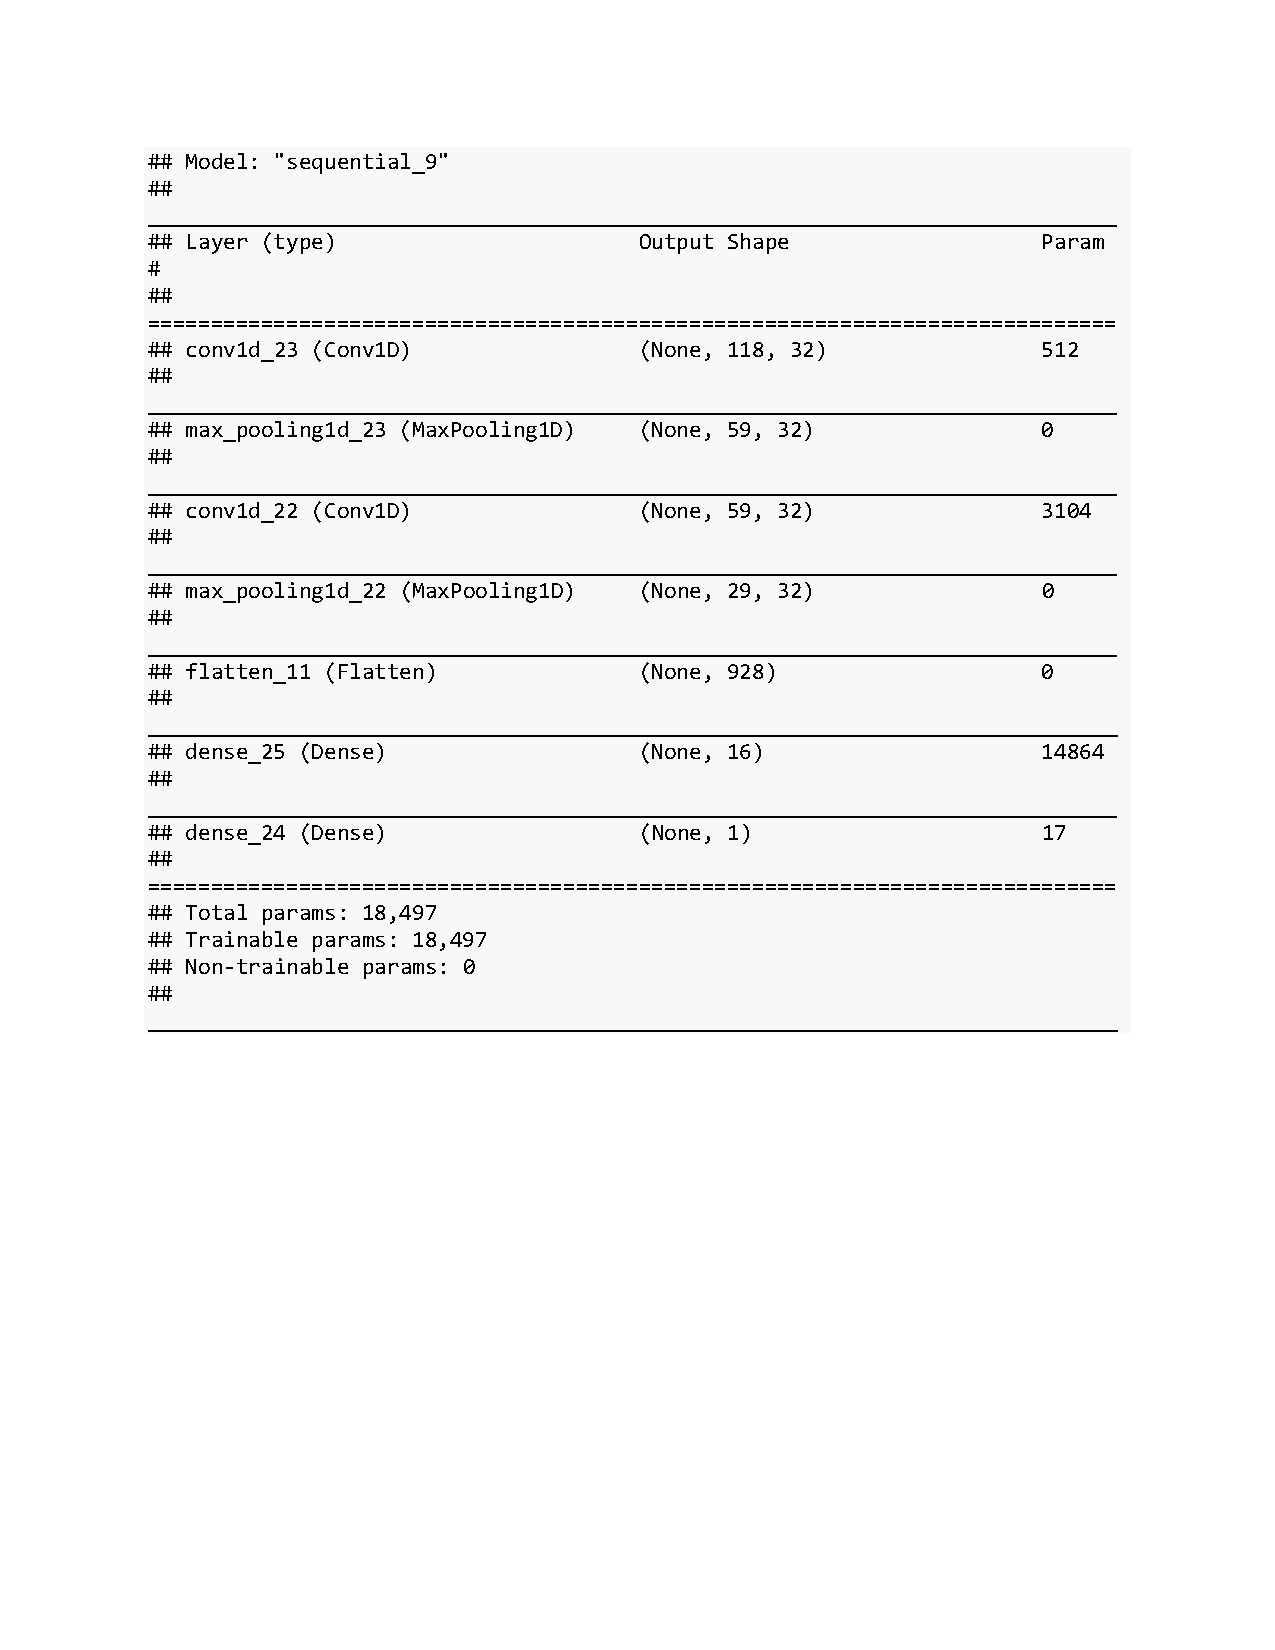
\includegraphics[scale=0.5]{Figures/summary_CNN_class_syn}
	\decoRule
	\caption[Experiment 1: Summary of CNNs for supervised learning]{Summary of CNN \parencite{own}}
	\label{fig:summary_CNN_class_syn}
\end{figure}

\begin{figure}[h]
	\centering
	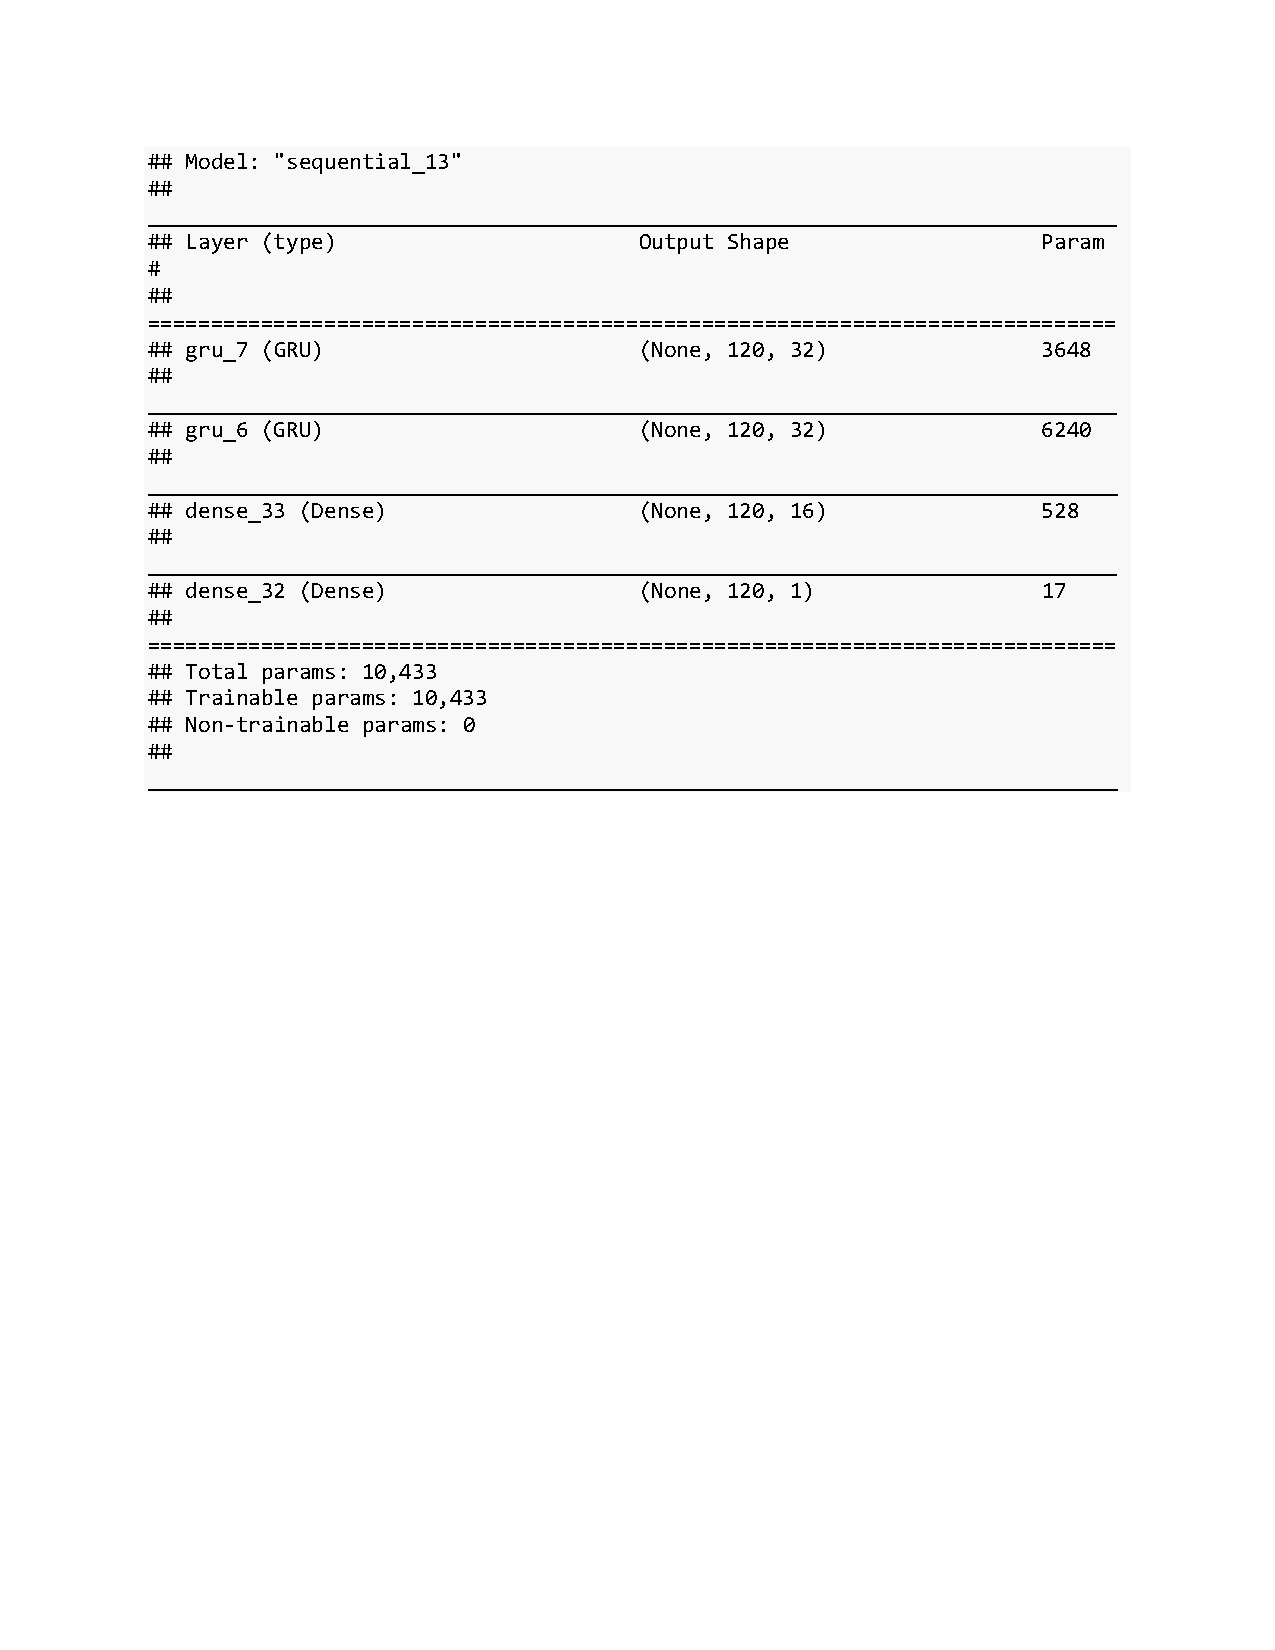
\includegraphics[scale=0.5]{Figures/summary_GRU_class_syn}
	\decoRule
	\caption[Experiment 1: Summary of GRU for supervised learning]{Summary of GRU \parencite{own}}
	\label{fig:summary_GRU_class_syn}
\end{figure}

\clearpage
\subsection{Unsupervised Learning}
\begin{figure}[h]
	\centering
	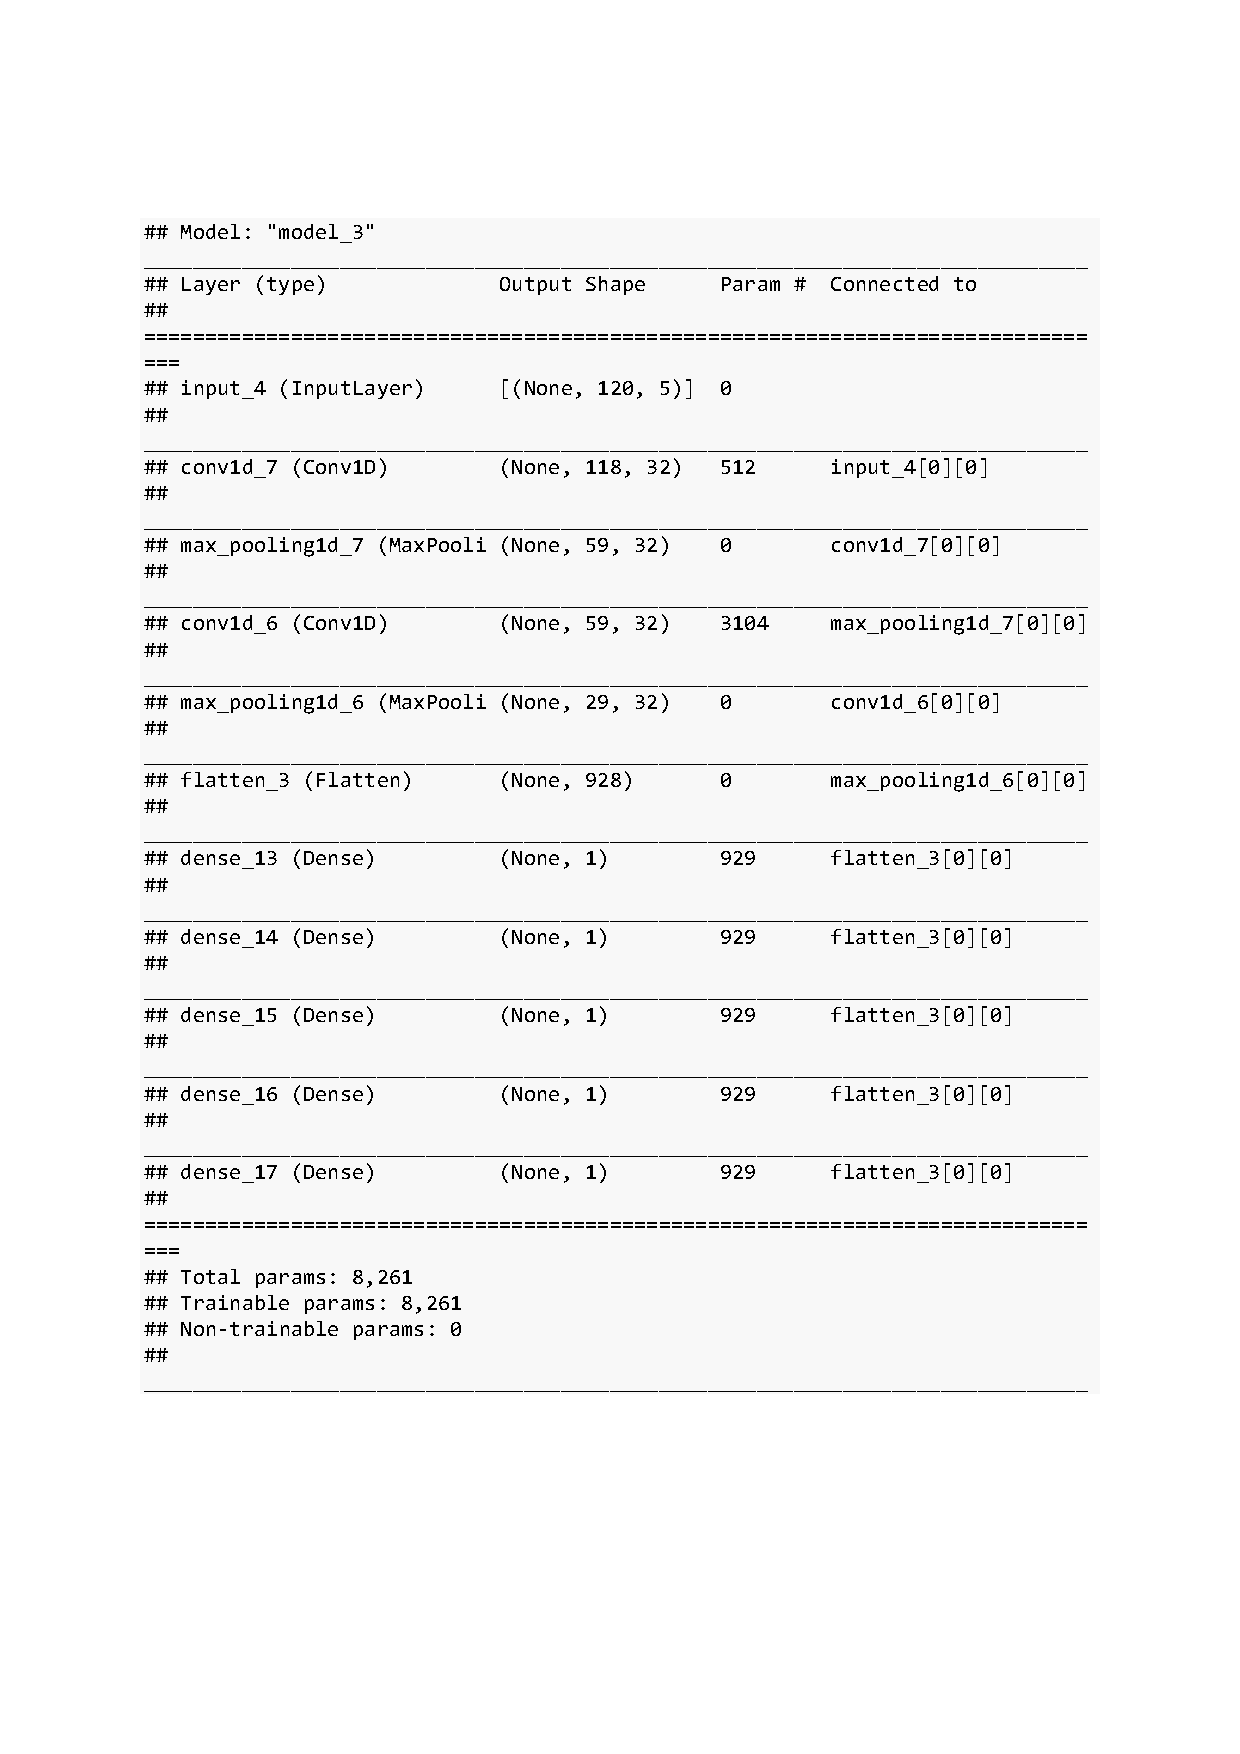
\includegraphics[scale=0.5]{Figures/summary_CNN_pred_syn}
	\decoRule
	\caption[Experiment 1: Summary of CNN for unsupervised learning]{Summary of CNN \parencite{own}}
	\label{fig:summary_CNN_pred_syn}
\end{figure}

\begin{figure}[h]
	\centering
	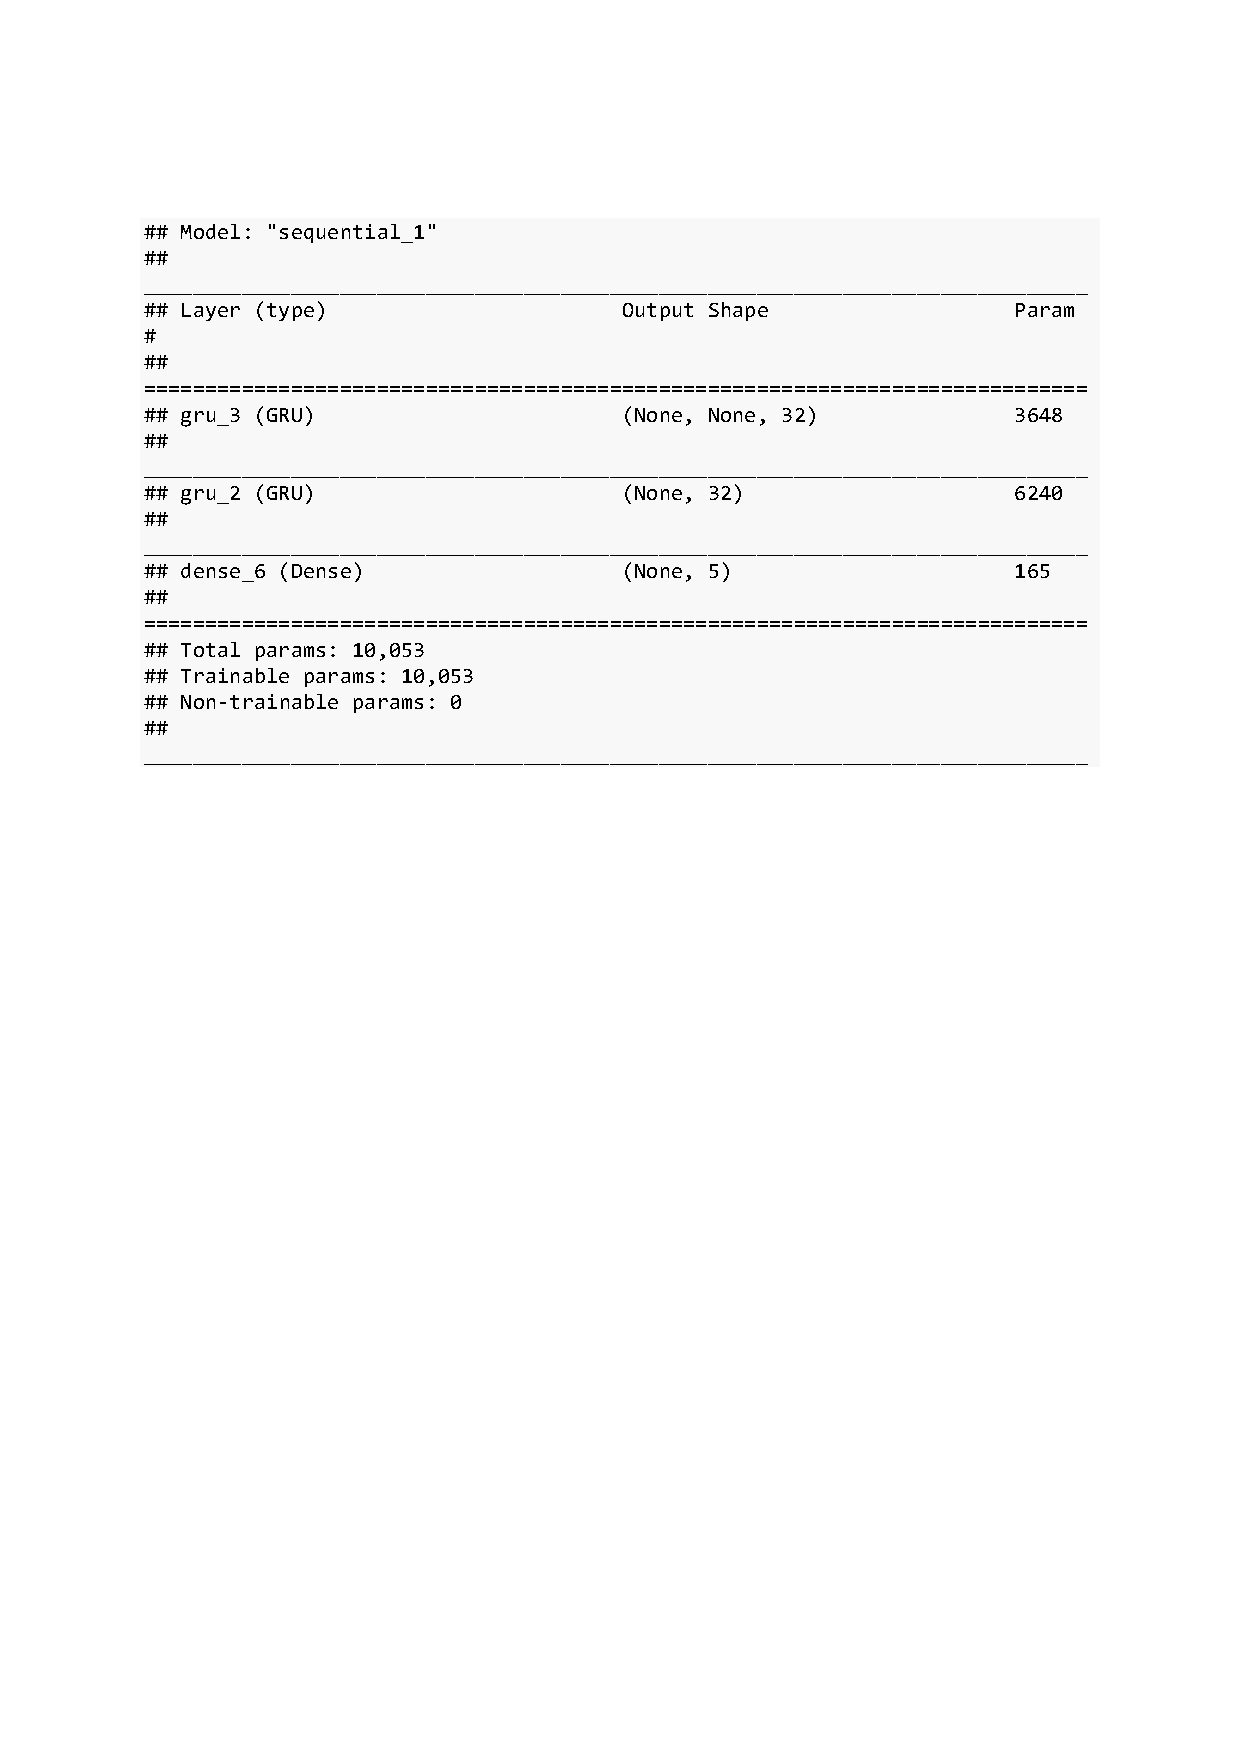
\includegraphics[scale=0.5]{Figures/summary_GRU_pred_syn}
	\decoRule
	\caption[Experiment 1: Summary of GRU for unsupervised learning]{Summary of GRU \parencite{own}}
	\label{fig:summary_GRU_pred_syn}
\end{figure}

\clearpage

\section{Summary of Models of Experiment 2}

\subsection{Supervised Learning}
%\begin{figure}[h]
%	\centering
%	\includegraphics[scale=0.5]{Figures/TBF}
%	\decoRule
%	\caption[Synthetic Anomalies]{Summary of CNN \parencite{own}}
%	\label{fig:CNN_classifier_house_temp}
%\end{figure}

\subsection{Unsupervised Learning}
\begin{figure}[h]
	\centering
	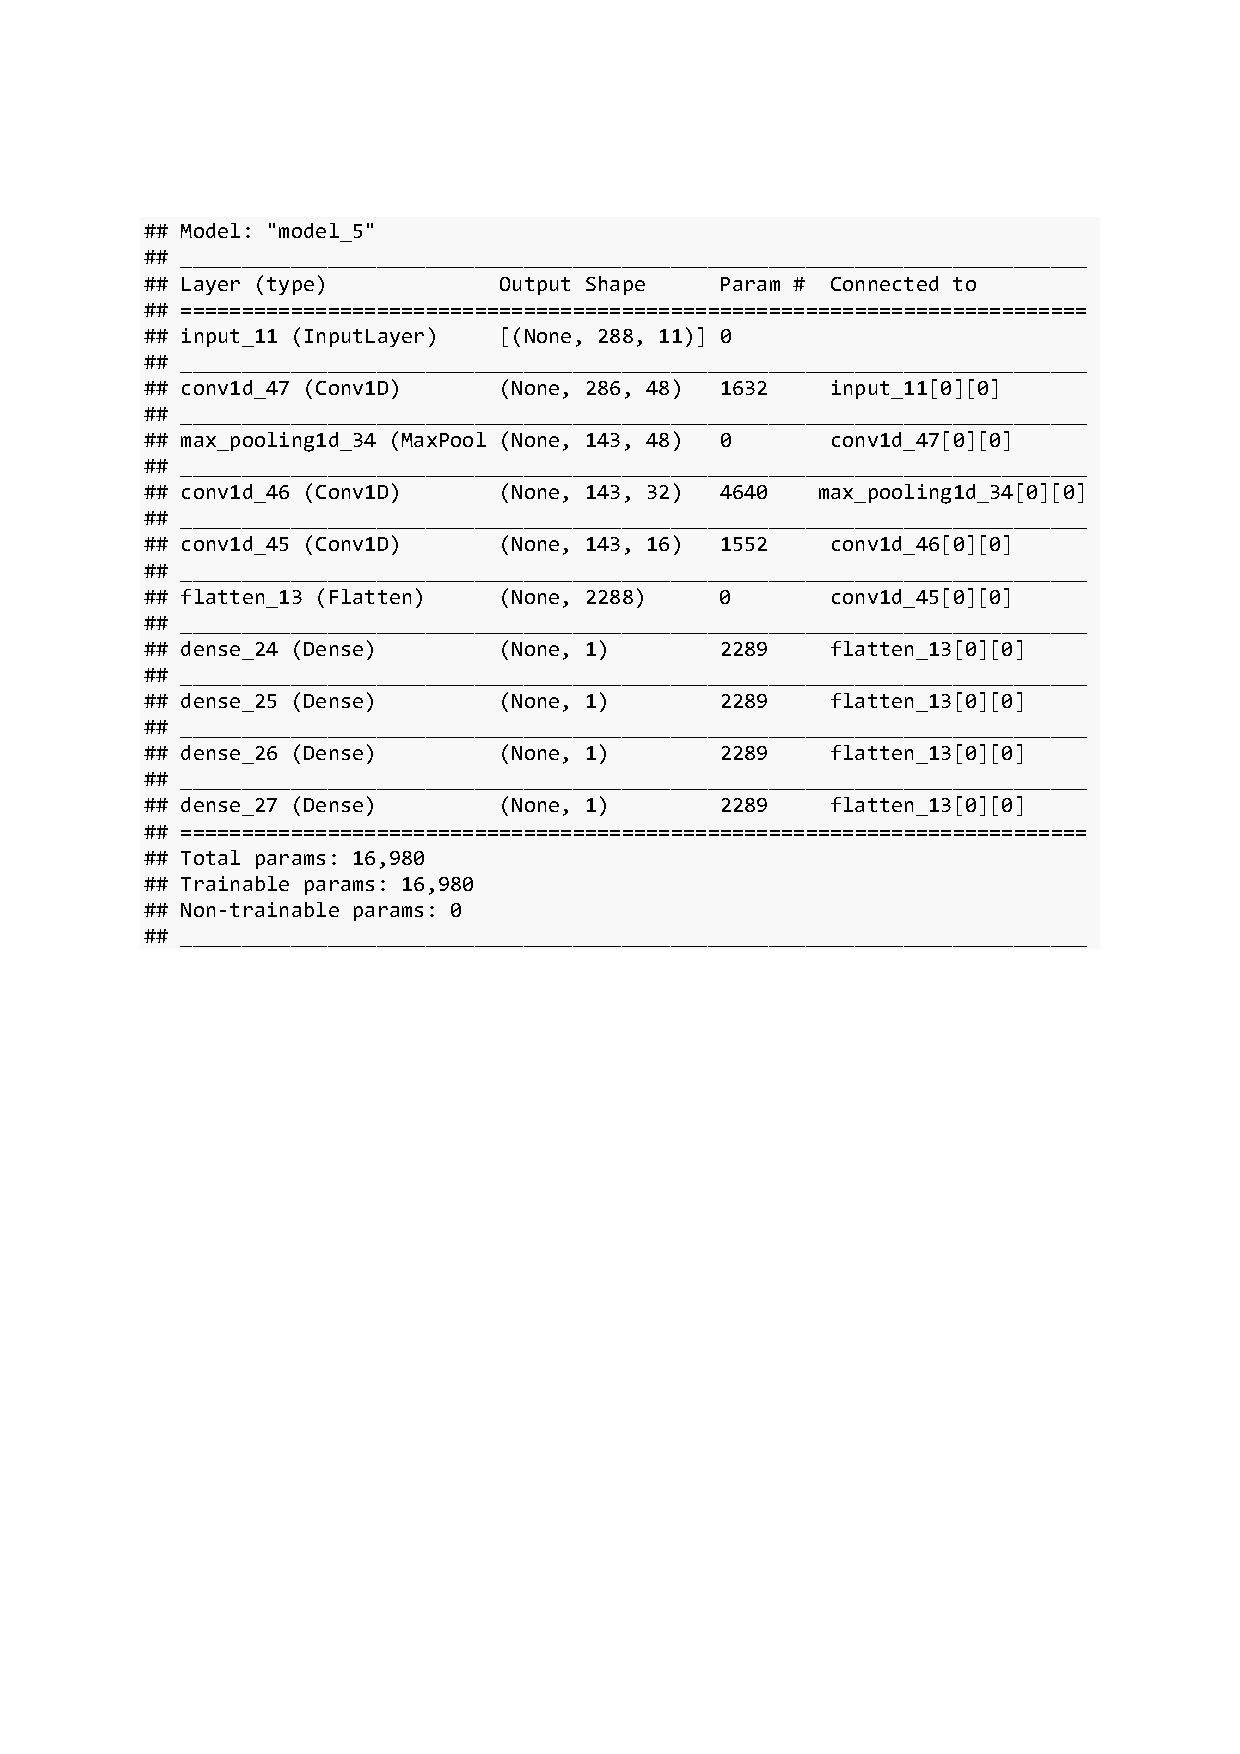
\includegraphics[scale=0.5]{Figures/summary_CNN_pred_house_temp}
	\decoRule
	\caption[Experiment 2: Summary of CNN for unsupervised learning]{Summary of CNN \parencite{own}}
	\label{fig:summary_CNN_pred_house_temp}
\end{figure}

\begin{figure}[h]
	\centering
	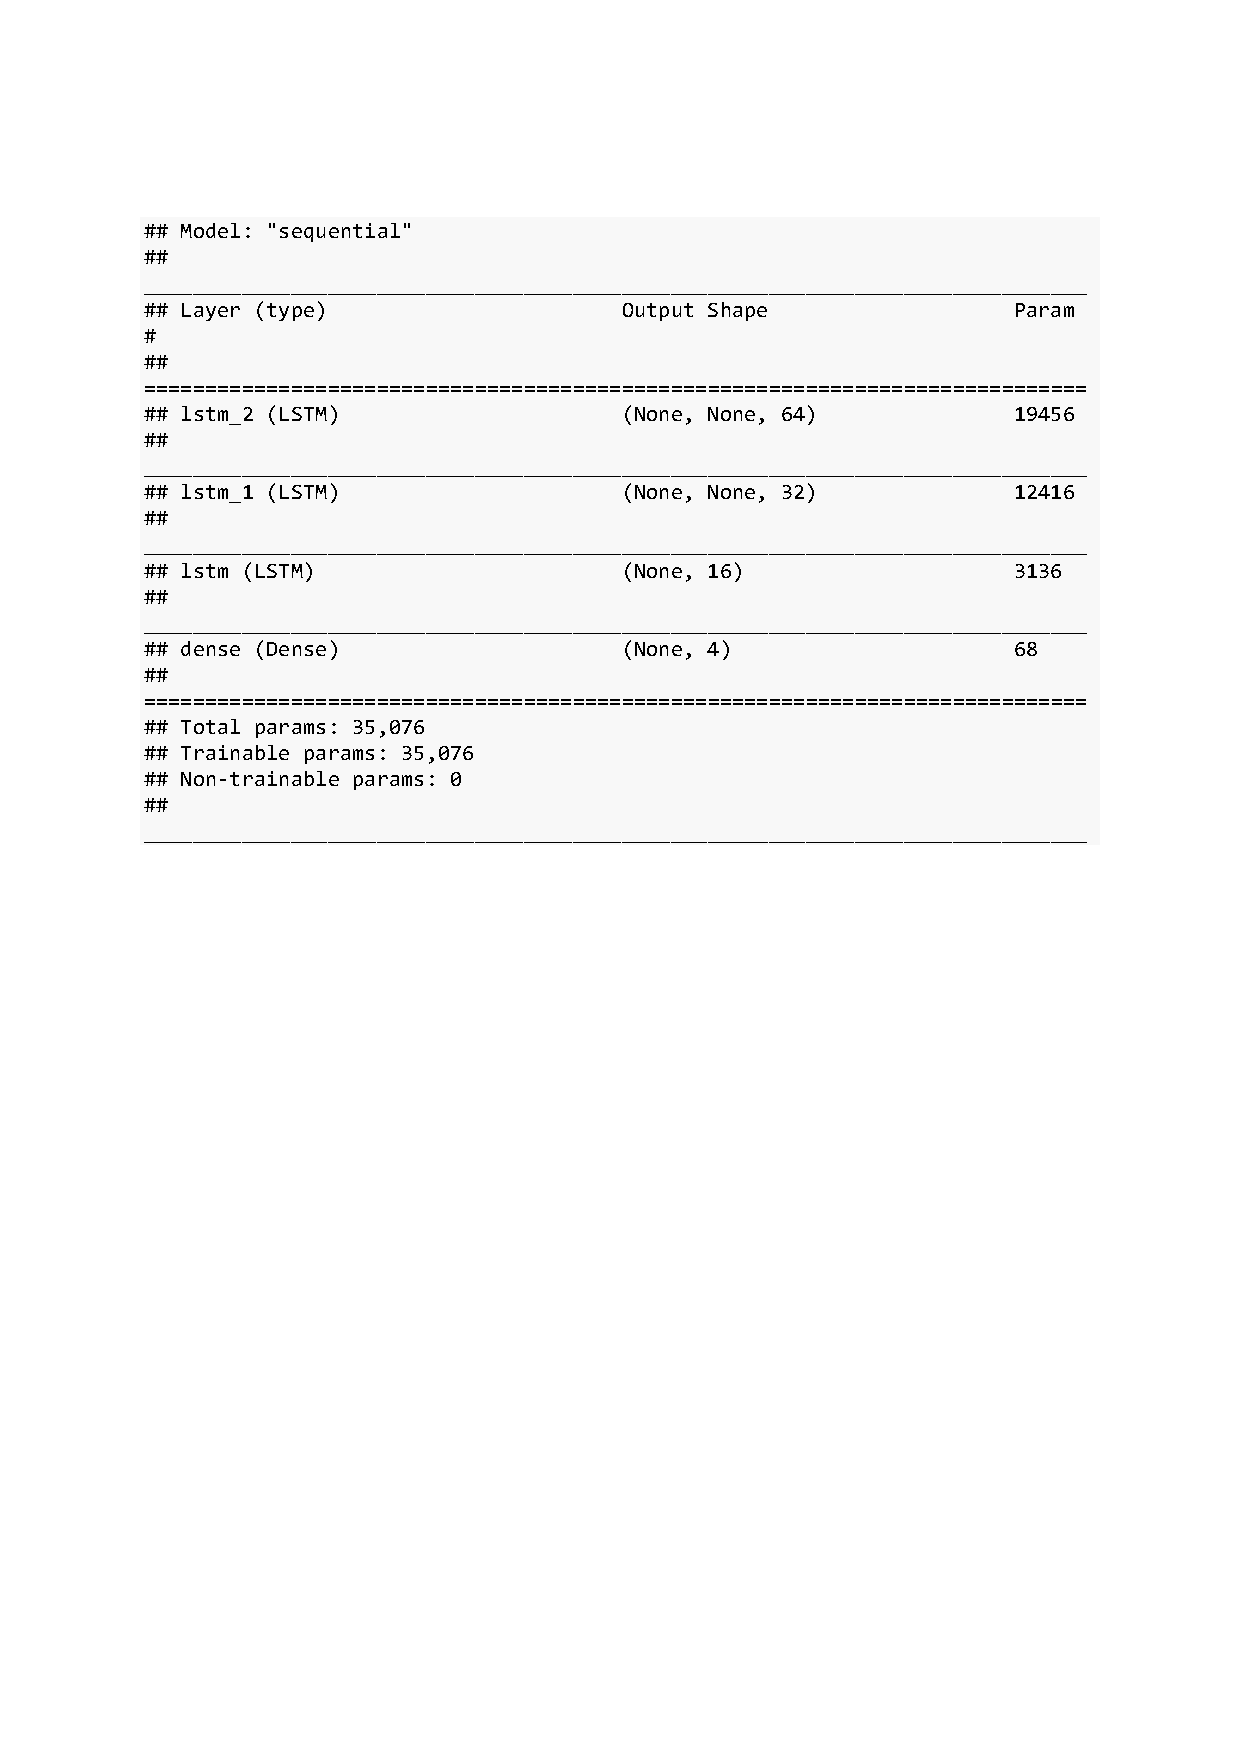
\includegraphics[scale=0.5]{Figures/summary_LSTM_pred_house_temp}
	\decoRule
	\caption[Experiment 2: Summary of LSTM for unsupervised learning]{Summary of LSTM \parencite{own}}
	\label{fig:summary_LSTM_pred_house_temp}
\end{figure}

\clearpage
\section{Summary of Models of Experiment 3}

\subsection{Unsupervised Learning}
\begin{figure}[h]
	\centering
	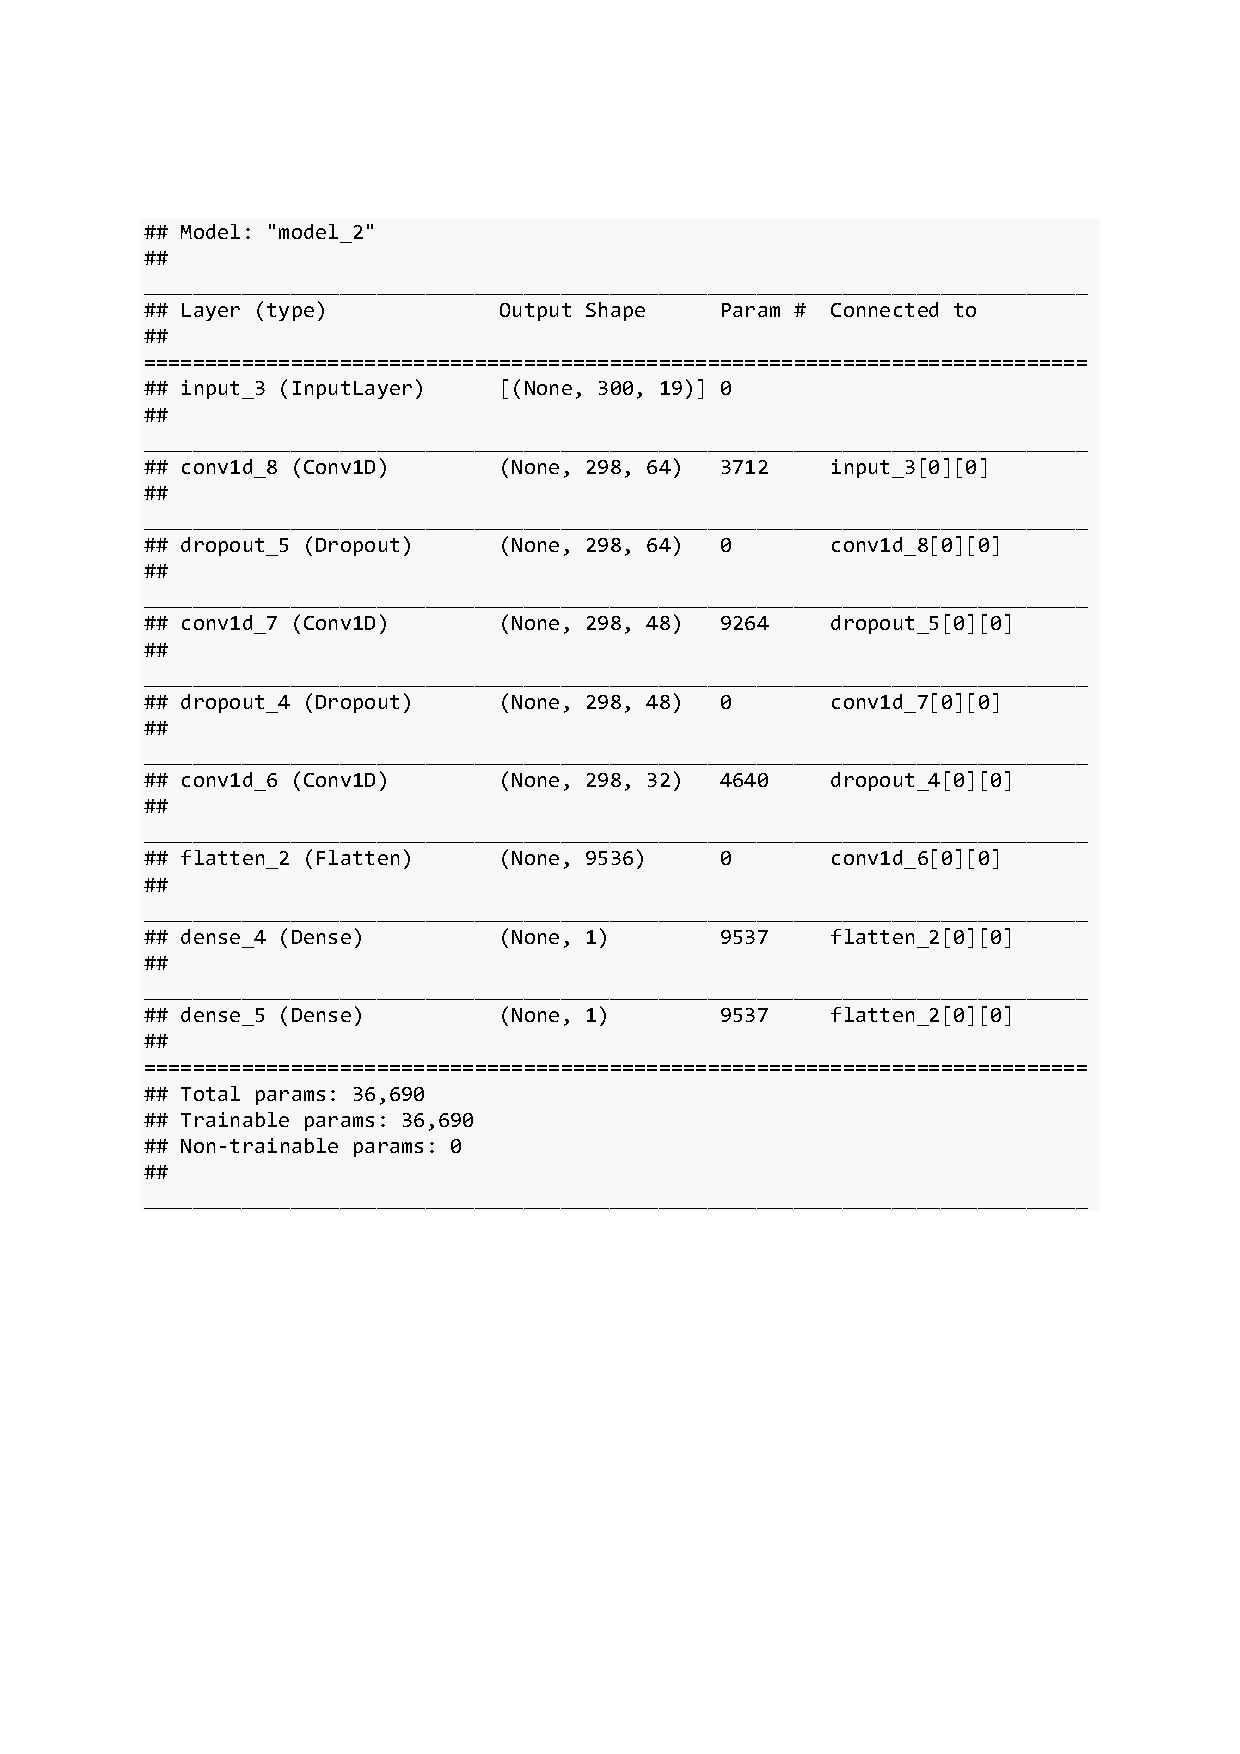
\includegraphics[scale=0.5]{Figures/summary_CNN_GHL}
	\decoRule
	\caption[Experiment 3: Summary of CNN for unsupervised learning]{Summary of CNN \parencite{own}}
	\label{fig:summary_CNN_GHL}
\end{figure}

\begin{figure}[h]
	\centering
	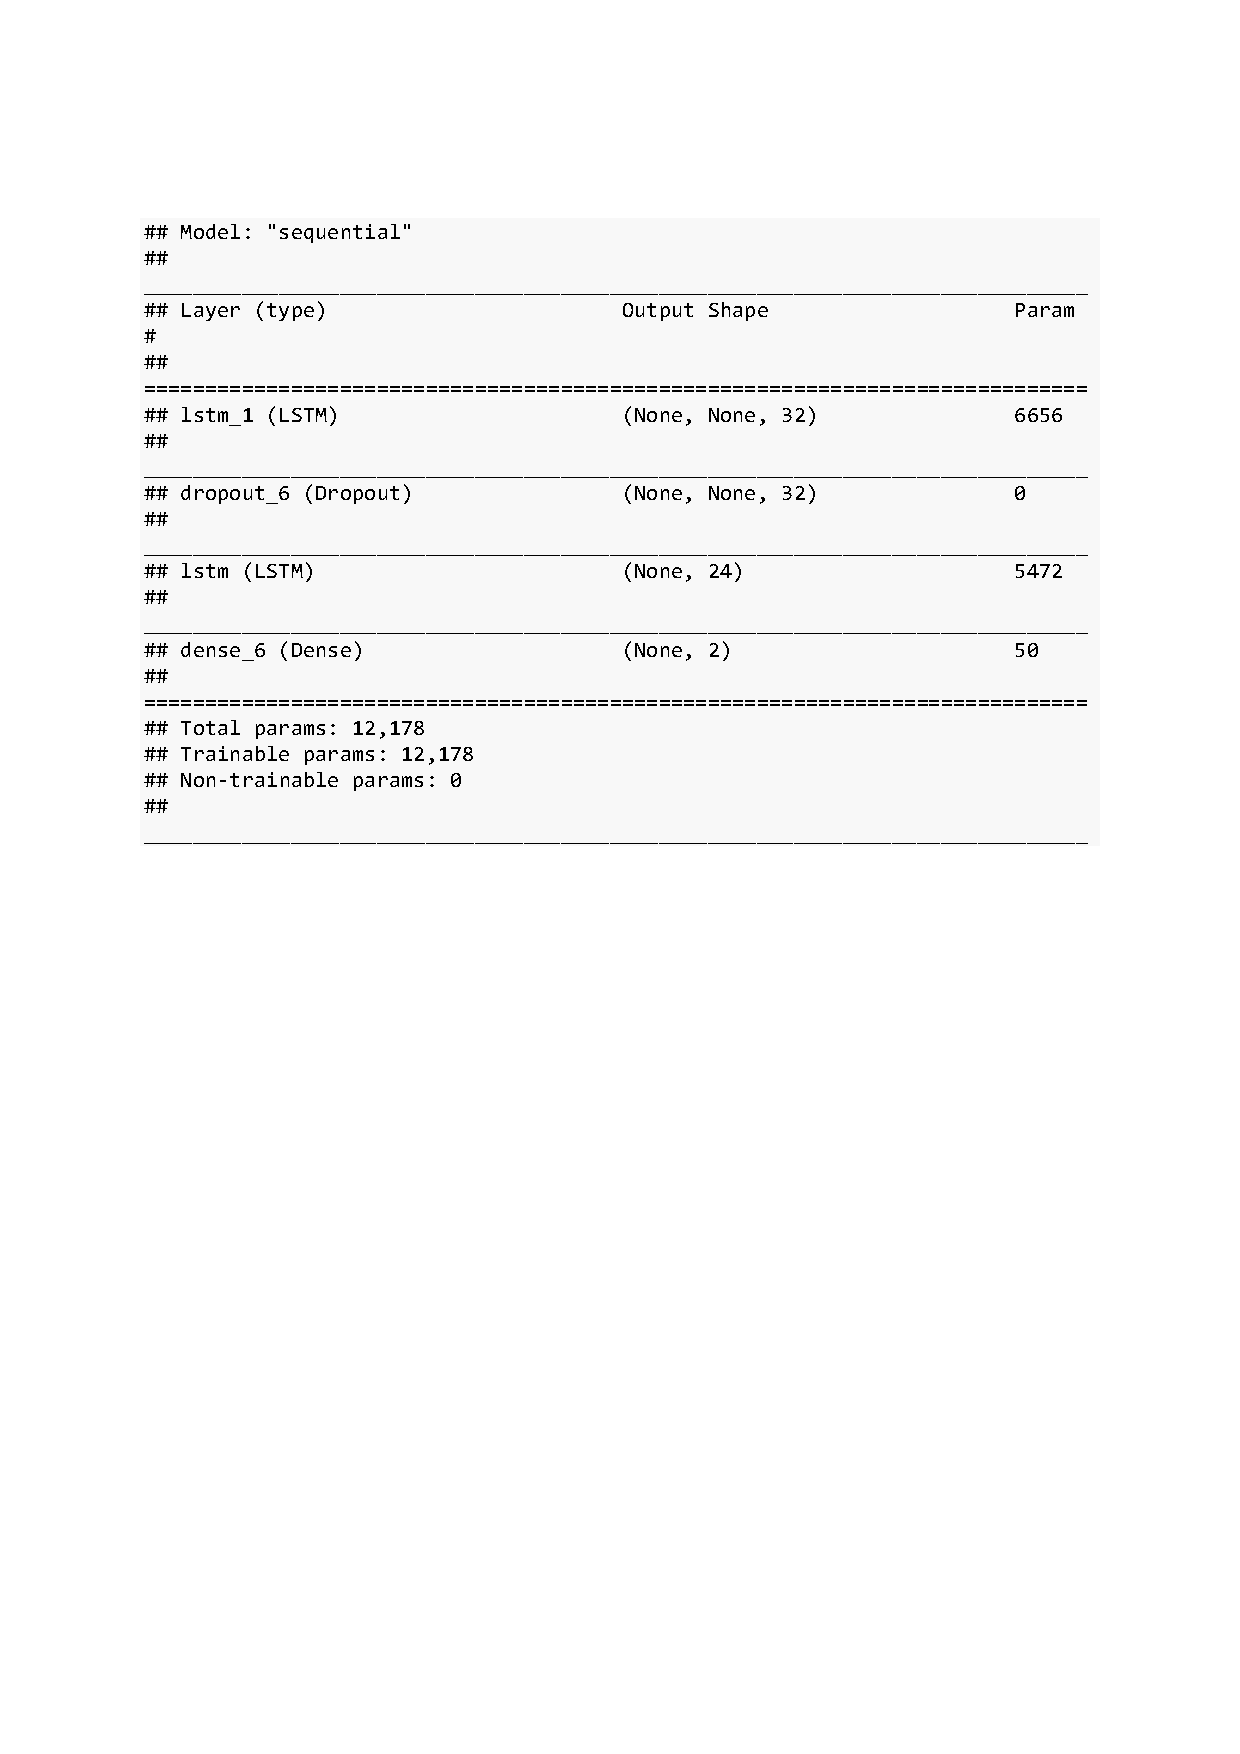
\includegraphics[scale=0.5]{Figures/summary_LSTM_GHL}
	\decoRule
	\caption[Experiment 3: Summary of LSTM for unsupervised learning]{Summary of LSTM \parencite{own}}
	\label{fig:summary_LSTM_GHL}
\end{figure}
%\include{Appendices/AppendixB}
%\include{Appendices/AppendixC}

%----------------------------------------------------------------------------------------
%	BIBLIOGRAPHY
%----------------------------------------------------------------------------------------

\printbibliography[heading=bibintoc]

%----------------------------------------------------------------------------------------

\end{document}  
